\documentclass[10pt,a4paper]{article}

%\documentclass[10pt,onecolumn,letterpaper]{IEEEtran}

\usepackage{setspace}
%\AtBeginDocument{\setstretch{.9}}
%\doublespacing  % doublespacing is done after title and before abstract

\usepackage{caption}
\usepackage{subcaption}
\usepackage[title]{appendix}
%
\usepackage[T1]{fontenc}
% T1 fonts will be used to generate the final print and online PDFs,
% so please use T1 fonts in your manuscript whenever possible.
% Other font encondings may result in incorrect characters.



\usepackage{graphicx}
% Used for displaying a sample figure. If possible, figure files should
% be included in EPS format.
%
% If you use the hyperref package, please uncomment the following two lines
% to display URLs in blue roman font according to Springer's eBook style:
%\usepackage{color}
%\renewcommand\UrlFont{\color{blue}\rmfamily}
%\urlstyle{rm}
%


% \usepackage{setspace}
%\AtBeginDocument{\setstretch{.9}}
%\doublespacing  % doublespacing is done after title and before abstract

\usepackage{caption}
\usepackage{subcaption}
\usepackage[title]{appendix}

\usepackage[margin=1in]{geometry}

%\usepackage{lineno}
%\linenumbers

% \usepackage{fullpage}
\usepackage{authblk}
\usepackage[utf8]{inputenc}
\usepackage{amsmath,bm}
\usepackage{amsthm}
\usepackage{amssymb}
\usepackage{hyperref}
\usepackage{adjustbox}
\usepackage{multirow}
\usepackage{graphicx}
\usepackage{booktabs}
\usepackage{caption}
\usepackage{subcaption}
\usepackage[table]{xcolor}
\usepackage{tabu}
\usepackage{subcaption}
\usepackage{longtable}
\usepackage{amssymb}
\usepackage{footnote}
\usepackage{hyperref}
\usepackage{multirow}
\usepackage{comment}
\usepackage{cite}
\usepackage{threeparttable}
\usepackage{makecell}
\usepackage{mathtools} % for multiline-multicase equation
\usepackage{float}
\usepackage{array}
\usepackage{tabularx} % in the preamble
\usepackage{tikz}
\usepackage{ulem}
\usepackage{algorithm2e}

\usepackage{tabularx}
\newcolumntype{Y}{>{\centering\arraybackslash}X}
\newcolumntype{C}[1]{>{\centering\arraybackslash}m{#1}}

\usepackage{xcolor}



\newcommand{\add}[1]{{\color{blue} #1}}
\newcommand{\addb}[1]{{\color{red} #1}}
\newcommand{\SR}[1]{{\color{red} #1}}
\newcommand{\methodname}{{\color{purple}Method\_Name~}}

% \newtheorem{theorem}{Theorem}[section]
% \newtheorem{corollary}{Corollary}[theorem]
% \newtheorem{lemma}[theorem]{Lemma}

% \renewcommand{\thetheorem}{\arabic{theorem}}  % to start numbering from 1

%\usepackage{booktabs, caption, makecell}
%\renewcommand\theadfont{\bfseries}
\usepackage{subfiles} % For subfiles
\usepackage{hyperref}
\usepackage[labelfont=bf]{caption}

\usepackage{xcolor}

\newcommand{\add}[1]{{\color{blue} #1}}
\newcommand{\addr}[1]{{\color{red} #1}}

\renewcommand\theadalign{bc}
\renewcommand\theadfont{\bfseries}
\renewcommand\theadgape{\Gape[4pt]}
\renewcommand\cellgape{\Gape[4pt]}

\makesavenoteenv{tabular}
\makesavenoteenv{table}

\hypersetup{
    urlcolor=blue,
}

%
\title{STELAR-X: Scaling Coalescent-Based Species Tree Inference to 100,000 Species and Beyond
\author[1,*]{Anik Saha$^{1}$ and Md. Shamsuzzoha Bayzid}
}

\affil[1]{Department of Computer Science and Engineering\protect\\Bangladesh University of Engineering and Technology, Dhaka-1205, Bangladesh}
\affil[*]{Corresponding author: shams\_bayzid@cse.buet.ac.bd}
\date{}





%Pushing the Boundaries of Phylogenomic Scale: STELAR-X Enables Coalescent-Based Species Tree Inference for 50,000 Species

%Ultra-Large and Statistically Consistent Species Tree Inference: STELAR-X Scales to 50,000 Species

%STELAR-X: Scaling Coalescent-Based Species Tree Inference to 1000,000 Species and Beyond

% %
% \titlerunning{QT-WEAVER}
% % If the paper title is too long for the running head, you can set
% % an abbreviated paper title here
% %
% \author{Navid Bin Hasan\inst{1,\dag}\orcidID{0009-0004-7792-9798} \and
% Sohaib\inst{1,\dag}\orcidID{0009-0003-8861-4743} \and
% Md. Shamsuzzoha Bayzid\inst{1}\orcidID{0000-0002-5640-0615}}
% %
% \authorrunning{N. Hasan et al.}
% % First names are abbreviated in the running head.
% % If there are more than two authors, 'et al.' is used.
% %
% \institute{\textsuperscript{1} Computer Science and Engineering, Bangladesh University of Engineering and Technology, Dhaka-1205, Bangladesh\\
% \textsuperscript{\dag} These authors contributed equally to this work
% \\
% \email{navidhasan0@gmail.com, sohaibbinmusa@gmail.com, shams\_bayzid@cse.buet.ac.bd}}





\begin{document}

\maketitle

\pagenumbering{gobble}

\begin{abstract}
%TBW
%\add{contributions we need to highlight in abstract/introduction: unprecedented scalibility; theoretical running time and memory usage improvement; $O(n^k)$ to $O(nk)$ memory usage using a novel and efficient representation of subtree-bipartitions. introduced a permutation-invariant and associative hash function with provable theoretical guarantee of negligible global collisions in order to ensure efficient mapping of the frequency of subtree-bipartitions. Efficient precomputation of bipartition weights with theoretical guarantee of ... GPU parallelization of pre-computing the weights efficiently.

%achieves comparable accuracy to state-of-the-art methods but with greater speed and lower memory use. Our method supports species tree estimation at scale and within minutes, which will be useful for many large phylogenomic studies.

Summary methods reconstruct species trees from collections of gene trees by accounting for gene tree discordance, and offer a statistically consistent framework for phylogenomic inference under the multispecies coalescent model.
While existing triplet- and quartet-based approaches such as ASTRAL and STELAR have provable statistical consistency, their running time and memory usage restrict their applicability to ultra-large datasets. We introduce STELAR-X, a highly scalable triplet-based phylogenetic inference algorithm that achieves an asymptotically optimal memory complexity of $O(nk)$ for \textit{n} species and \textit{k} gene trees--essentially matching the input size and allowing analyses to remain feasible as long as the input trees fit in memory--while also substantially reducing running time. STELAR-X introduces a novel, compact integer tuple-based encoding of tree bipartitions along with a customized double hashing scheme using permutation-invariant and associative hash functions with a provably negligible global collision probability. This representation enables efficient computation of bipartition weights and underpins a dynamic programming algorithm with substantially reduced computational overhead.
We further leverage GPU parallelism for fast precomputation of bipartition weights. Extensive experiments demonstrate that STELAR-X preserves the  accuracy of STELAR while scaling to unprecedented dataset sizes. On simulated datasets with 5,000 taxa and 1,000 gene trees, STELAR-X runs 445$\times$ faster than ASTRAL-MP (the most scalable version of ASTRAL) while using 9$\times$ less CPU memory. Most significantly, STELAR-X analyzed a dataset of 100,000 taxa and 1,000 genes in  8.5 hours using 86 GB RAM, and a 100,000-gene dataset with 1000 taxa in just 4 minutes using 106 GB RAM -- scales that were previously intractable for statistically consistent summary methods. STELAR-X is publicly available at \url{https://github.com/aaniksahaa/STELAR-X}.

%establishes a new benchmark for ultra-large phylogenomic inference. %is the first statistically consistent summary method that can analyze datasets with  100,000 taxa and thousands of genes in only 8.5 hours using 86 GB of RAM, establishing a new benchmark for large-scale phylogenomic inference.

%\addr{100,000 genes}

%\textcolor{blue}{Sir, 1000 taxa, 100,000 genes took 106 GB RAM but ran only within 4 minutes (235.06 s). May we also add it in the abstract?}

%\keywords{Species tree \and Gene tree \and Incomplete lineage sorting (ILS) \and Quartet distribution \and Quartet consistency.}
\end{abstract}
\clearpage
\pagenumbering{arabic}

\newcommand{\quartet}[4]{
  \begin{tikzpicture}
    % Nodes
    \node (a) at (0, 2) {};
    \node (b) at (0, 0) {};
    \node (c) at (3, 2) {};
    \node (d) at (3, 0) {};
    \node (center1) at (1, 1) {};
    \node (center2) at (2, 1) {};
    \node (name) at (1.5, -0.5) {$#1#2|#3#4$};

    % Edges
    \draw[thick] (a) -- (center1);
    \draw[thick] (b) -- (center1);
    \draw[thick] (center1) -- (center2);
    \draw[thick] (center2) -- (c);
    \draw[thick] (center2) -- (d);

    % Dots at nodes
    \fill (a) circle (2pt);
    \fill (b) circle (2pt);
    \fill (c) circle (2pt);
    \fill (d) circle (2pt);
    \fill (center1) circle (2pt);
    \fill (center2) circle (2pt);

    % Labels
    \node at (-0.2, 2) {#1};
    \node at (3.2, 2) {#3};
    \node at (3.2, 0) {#4};
    \node at (-0.2, 0) {#2};
  \end{tikzpicture}
}

\newcommand{\fivetax}[5]{
\begin{tikzpicture}
% Nodes
\node (a) at (0, 2) {};
\node (b) at (0, 0) {};
\node (c) at (3, 2) {};
\node (d) at (3, 0) {};
\node (x) at (0.5, 1.5) {};
\node (e) at (0, 1) {};

\node (center1) at (1, 1) {};
\node (center2) at (2, 1) {};

% Edges
\draw[thick] (a) -- (x);
\draw[thick] (center1) -- (x);
\draw[thick] (b) -- (center1);
\draw[thick] (center1) -- (center2);
\draw[thick] (center2) -- (c);
\draw[thick] (center2) -- (d);
\draw[thick] (e) -- (x);

% Dots at nodes
\fill (a) circle (2pt);
\fill (b) circle (2pt);
\fill (c) circle (2pt);
\fill (d) circle (2pt);
\fill (x) circle (2pt);
\fill (e) circle (2pt);
\fill (center1) circle (2pt);
\fill (center2) circle (2pt);

% Labels
\node at (-0.2, 2) {#1};
\node at (3.2, 2) {#3};
\node at (3.2, 0) {#4};
\node at (-0.2, 0) {#2};
\node at (-0.2, 1) {#5};
\end{tikzpicture}
}

\newcommand{\fivetaxcol}[5]{
\begin{tikzpicture}
% Nodes
\node (a) at (0, 2) {};
\node (b) at (0, 0) {};
\node (c) at (3, 2) {};
\node (d) at (3, 0) {};
\node (x) at (0.5, 1.5) {};
\node (e) at (0, 1) {};

\node (center1) at (1, 1) {};
\node (center2) at (2, 1) {};

% Edges
\draw[thick] (a) -- (x);
\draw[thick] (center1) -- (x);
\draw[thick] (b) -- (center1);
\draw[thick] (center1) -- (center2);
\draw[thick] (center2) -- (c);
\draw[thick] (center2) -- (d);
\draw[thick, red] (e) -- (x);


% Dots at nodes
\fill (a) circle (2pt);
\fill (b) circle (2pt);
\fill (c) circle (2pt);
\fill (d) circle (2pt);
\fill (x) circle (2pt);
% \fill[red] (e) circle (2pt);
\fill (e) circle (2pt);
\fill (center1) circle (2pt);
\fill (center2) circle (2pt);

% Labels
\node at (-0.2, 2) {#1};
\node at (3.2, 2) {#3};
\node at (3.2, 0) {#4};
\node at (-0.2, 0) {#2};
\node at (-0.2, 1) {#5};
\end{tikzpicture}
}

\newcommand{\fivetaxinv}[5]{
\begin{tikzpicture}
% Nodes
\node (a) at (0, 2) {};
\node (b) at (0, 0) {};
\node (c) at (3, 2) {};
\node (d) at (3, 0) {};
\node (x) at (0.5, 0.5) {};
\node (e) at (0, 1) {};

\node (center1) at (1, 1) {};
\node (center2) at (2, 1) {};

% Edges
\draw[thick] (a) -- (center1);
\draw[thick] (center1) -- (x);
\draw[thick] (b) -- (x);
\draw[thick] (center1) -- (center2);
\draw[thick] (center2) -- (c);
\draw[thick] (center2) -- (d);
\draw[thick] (e) -- (x);

% Dots at nodes
\fill (a) circle (2pt);
\fill (b) circle (2pt);
\fill (c) circle (2pt);
\fill (d) circle (2pt);
\fill (x) circle (2pt);
\fill (e) circle (2pt);

\fill (center1) circle (2pt);
\fill (center2) circle (2pt);

% Labels
\node at (-0.2, 2) {#1};
\node at (3.2, 2) {#3};
\node at (3.2, 0) {#4};
\node at (-0.2, 0) {#2};
\node at (-0.2, 1) {#5};
\end{tikzpicture}
}

\newcommand{\fivetaxmult}[5]{
\begin{tikzpicture}
% Nodes
\node (a) at (0, 2) {};
\node (b) at (0, 0) {};
\node (c) at (3, 2) {};
\node (d) at (3, 0) {};
\node (x) at (2.5, 0.5) {};
\node (x2) at (2.5, 1.5) {};
\node (x3) at (1.5, 1) {};
\node (y) at (0.5, 1.5) {};
\node (e) at (3, 1) {};
\node (e2) at (2, 2) {};
\node (e3) at (1.5, 0) {};

\node (center1) at (1, 1) {};
\node (center2) at (2, 1) {};

% Edges
\draw[thick] (a) -- (center1);
\draw[thick] (center1) -- (b);
% \draw[thick] (b) -- (x);
\draw[thick] (center1) -- (center2);
\draw[thick] (center2) -- (c);
\draw[thick] (center2) -- (d);

\draw[thick, dotted, red, shorten <=-1mm, shorten >=-1mm] (e) -- (x);
\draw[thick, dotted, red, shorten <=-1mm, shorten >=-1mm] (e2) -- (x2);
\draw[thick, dotted, red, shorten <=-1mm, shorten >=-1mm] (e3) -- (x3);


% Dots at nodes
\fill (a) circle (2pt);
\fill (b) circle (2pt);
\fill (c) circle (2pt);
\fill (d) circle (2pt);
% \fill (x) circle (2pt);
\fill (e) circle (2pt);
\fill (e2) circle (2pt);
\fill (e3) circle (2pt);
\fill (center1) circle (2pt);
\fill (center2) circle (2pt);

% Labels
\node at (-0.2, 2) {#1};
\node at (3.2, 2) {#3};
\node at (3.2, 0) {#4};
\node at (-0.2, 0) {#2};
\node at (3.2, 1) {#5};
\node at (1.8, 2) {#5};
\node at (1.7, 0) {#5};
\end{tikzpicture}
}







\newcommand{\fivetaxdccol}[5]{
\begin{tikzpicture}
% Nodes
\node (a) at (0, 2) {};
\node (b) at (0, 0) {};
\node (c) at (3, 2) {};
\node (d) at (3, 0) {};
\node (x) at (2.5, 0.5) {};
\node (x2) at (2.5, 1.5) {};
\node (x3) at (1.5, 1) {};
\node (y) at (0.5, 1.5) {};
\node (e) at (3, 1) {};
\node (e2) at (2, 2) {};
\node (e3) at (1.5, 0) {};

\node (center1) at (1, 1) {};
\node (center2) at (2, 1) {};

% Edges
\draw[thick] (a) -- (center1);
\draw[thick] (center1) -- (b);
% \draw[thick] (b) -- (x);
\draw[thick] (center1) -- (center2);
\draw[thick] (center2) -- (c);
\draw[thick] (center2) -- (x);
\draw[thick] (x) -- (d);

\draw[thick, red] (e) -- (x);



% Dots at nodes
\fill (a) circle (2pt);
\fill (b) circle (2pt);
\fill (c) circle (2pt);
\fill (d) circle (2pt);
% \fill (x) circle (2pt);
% \fill[red] (e) circle (2pt);
\fill (e) circle (2pt);
\fill (center1) circle (2pt);
\fill (center2) circle (2pt);
\fill (x) circle (2pt);

% Labels
\node at (-0.2, 2) {#1};
\node at (3.2, 2) {#3};
\node at (3.2, 0) {#4};
\node at (-0.2, 0) {#2};
\node at (3.2, 1) {#5};
% \node at (1.8, 2) {#5};
% \node at (1.7, 0) {#5};
\end{tikzpicture}
}

\newcommand{\fivetaxdc}[5]{
\begin{tikzpicture}
% Nodes
\node (a) at (0, 2) {};
\node (b) at (0, 0) {};
\node (c) at (3, 2) {};
\node (d) at (3, 0) {};
\node (x) at (2.5, 0.5) {};
\node (x2) at (2.5, 1.5) {};
\node (x3) at (1.5, 1) {};
\node (y) at (0.5, 1.5) {};
\node (e) at (3, 1) {};
\node (e2) at (2, 2) {};
\node (e3) at (1.5, 0) {};

\node (center1) at (1, 1) {};
\node (center2) at (2, 1) {};

% Edges
\draw[thick] (a) -- (center1);
\draw[thick] (center1) -- (b);
% \draw[thick] (b) -- (x);
\draw[thick] (center1) -- (center2);
\draw[thick] (center2) -- (c);
\draw[thick] (center2) -- (x);
\draw[thick] (x) -- (d);

\draw[thick, shorten <=-1mm, shorten >=-1mm] (e) -- (x);



% Dots at nodes
\fill (a) circle (2pt);
\fill (b) circle (2pt);
\fill (c) circle (2pt);
\fill (d) circle (2pt);
% \fill (x) circle (2pt);
\fill (e) circle (2pt);
\fill (center1) circle (2pt);
\fill (center2) circle (2pt);
\fill (x) circle (2pt);

% Labels
\node at (-0.2, 2) {#1};
\node at (3.2, 2) {#3};
\node at (3.2, 0) {#4};
\node at (-0.2, 0) {#2};
\node at (3.2, 1) {#5};
% \node at (1.8, 2) {#5};
% \node at (1.7, 0) {#5};
\end{tikzpicture}
}


\newcommand{\triplet}[4]{
\begin{tikzpicture}
% Nodes
\node (a) at (0, 2) {};
\node (b) at (0, 0) {};
\node (center1) at (1, 1) {};
\node (c) at (2.5, 1) {};
\node (x) at (0.5, 0.5) {};
\node (y) at (0.5, 1.5) {};
\node (z) at (1.75, 1) {};
\node (d1) at (0, 1) {};
\node (d2) at (1, 2) {};
\node (d3) at (1.75, 0) {};

% Edges
\draw[thick] (a) -- (center1);
\draw[thick] (center1) -- (b);
\draw[thick] (center1) -- (c);

\draw[thick, dotted, red, shorten <=-1mm, shorten >=-1mm] (d1) -- (x);
\draw[thick, dotted, red, shorten <=-1mm, shorten >=-1mm] (d2) -- (y);
\draw[thick, dotted, red, shorten <=-1mm, shorten >=-1mm] (d3) -- (z);


% Dots at nodes
\fill (a) circle (2pt);
\fill (b) circle (2pt);
\fill (c) circle (2pt);
\fill (d1) circle (2pt);
\fill (d2) circle (2pt);
\fill (d3) circle (2pt);
\fill (center1) circle (2pt);

% Labels
\node at (-0.2, 2) {#1};
\node at (2.7, 1) {#3};
\node at (-0.2, 1) {#4};
\node at (1.2, 2) {#4};
\node at (1.95, 0) {#4};
\node at (-0.2, 0) {#2};
% \node at (3.2, 1) {#5};
% \node at (1.8, 2) {#5};
% \node at (1.7, 0) {#5};
\end{tikzpicture}
}


\newcommand{\linequart}[6]{
\begin{tikzpicture}
% Nodes
\node (a) at (0, 0) {};
\node (b) at (6, 0) {};
\node (cx) at (1.2, 0) {};
\node (xx) at (2.4, 0) {};
\node (dx) at (3.6, 0) {};
\node (yx) at (4.8, 0) {};

\node (c) at (1.2, 1) {};
\node (d) at (3.6, 1) {};
\node (x) at (2.4, -1) {};
\node (y) at (4.8, -1) {};

% Edges
\draw[thick] (a) -- (b);
\draw[dashed] (c) -- (cx);
\draw[dashed] (d) -- (dx);
\draw[dashed] (x) -- (xx);
\draw[dashed] (y) -- (yx);

% Dots at nodes
\fill (a) circle (2pt);
\fill (b) circle (2pt);
\fill (cx) circle (1.2pt);
\fill (dx) circle (1.2pt);
\fill (xx) circle (1.2pt);
\fill (yx) circle (1.2pt);
\fill (c) circle (1.5pt);
\fill (d) circle (1.5pt);
\fill (x) circle (1.5pt);
\fill (y) circle (1.5pt);

% Labels
\node at (-0.2, 0) {#1};
\node at (6.2, 0) {#2};
\node at (1, 1) {#3};
\node at (3.4, 1) {#4};
\node at (2.6, -1) {#5};
\node at (5, -1) {#6};

\end{tikzpicture}
}

\section{Introduction}

Widespread genome-wide discordance poses a major challenge for phylogenomic studies based on multi-locus datasets~\cite{jarvis2014,1kp}. A species tree represents the branching pattern of species through speciation events, while a gene tree describes the evolutionary history of a particular gene across those species. Various biological processes can cause different loci to follow different evolutionary paths, so estimating a species tree typically involves analyzing multiple genes and alignments across the genome. Among these processes, incomplete lineage sorting (ILS) is widely recognized as a dominant source of discordance, best explained under the multispecies coalescent model~\cite{Hud83,Nei86,Nei87,Rosenberg02}. In the presence of gene tree heterogeneity, traditional approaches such as concatenation--where gene alignments are merged into a single supermatrix to infer one tree--can be statistically inconsistent~\cite{roch2015likelihood,consensus-inconsistent}, and produce incorrect trees with high support~\cite{kubatko-degnan-2007}.

To overcome these limitations, a range of methods have been developed that explicitly account for ILS, many of which are provably statistically consistent, meaning that they will converge in probability to the true species tree given sufficiently large numbers of genes and sites per gene~\cite{heled-drummond,BEAST,best,svdquartet,mpest}. The most scalable among these are ``summary methods'', which first infer gene trees for individual loci and then combine them to estimate the species tree. Notable examples of statistically consistent, coalescent-based summary methods include MP-EST~\cite{mpest}, ASTRAL~\cite{astral}, BUCKy~\cite{larget-bioinf2010}, GLASS~\cite{glass}, STEM~\cite{stem}, SVDquartet~\cite{svdquartet},
STEAC~\cite{steac}, NJst~\cite{njst}, ASTRID~\cite{astrid}, 
STELAR~\cite{stelar}.

Among summary methods, ASTRAL has emerged as the most widely used and accurate approach for large-scale phylogenomic analyses under the multispecies coalescent model. By maximizing quartet consistency across input gene trees, ASTRAL provides statistically consistent species tree estimates. ASTRAL and its parallel implementation ASTRAL-MP~\cite{astral-mp} have been shown to scale to datasets with up to $\sim$10,000 species with several days of running time. Despite these advances, both ASTRAL and ASTRAL-MP face scalability bottlenecks when the number of species and genes exceeds several tens of thousands.

Improving the scalability of species tree inference has long been a key focus in phylogenomics. Divide-and-conquer strategies have proven particularly effective in extending summary methods to larger datasets. For example, the disk-covering method~\cite{dcm-boosting}  demonstrated that partitioning taxa into overlapping subsets (``disks''), inferring local trees, and merging them can substantially enhance scalability without sacrificing accuracy. %Building on the spirit of such hierarchical approaches, recent methods have sought to further extend scalability to tens of thousands of taxa.
A notable recent development in this direction is uDANCE~\cite{udance}, a divide-and-conquer framework for inferring and incrementally updating large genome-wide phylogenetic trees. Unlike traditional phylogenomic methods that reconstruct trees \textit{de novo} each time, uDance can  update and expand an existing ``backbone'' tree as new genomes are added. %In doing so, uDANCE departs from traditional summary methods (such as ASTRAL) that operate by directly optimizing quartet scores across gene tree inputs for all taxa simultaneously. 
The backbone-growth paradigm allows uDANCE to analyze much larger taxon sets than standard  summary methods. However, constructing a  ``tree of life'' may require building backbone trees consisting of hundreds of thousands of taxa--a challenge that remains unresolved. Furthermore, because uDANCE is not explicitly designed to ensure statistical consistency under the multispecies coalescent model, the scalability of provably consistent summary methods (e.g., ASTRAL) still falls far short of the needs of ultra-large phylogenomics involving hundreds of thousands of species.

In this work, we address this gap by introducing STELAR-X, an extended version of the statistically consistent, coalescent-based method STELAR (Species Tree Estimation by maximizing tripLet AgReement)~\cite{stelar}. STELAR-X achieves unprecedented scalability through a combination of algorithmic redesign and efficient data representations. 
%a novel, compact tuple-based representation of subtree bipartitions that avoids prohibitive  bitset storage
We introduce a new, compact integer tuple-based representation of tree bipartitions that avoids traditional $O(n^2k)$ bitset-based encoding used in widely used methods like ASTRAL (\addr{Anik: confirm that ASTRAL uses bitset operations}). We also used a customized double-hashing scheme based on associative hash functions with provably negligible collision probability. In addition, we introduce optimized CPU and GPU parallelization to accelerate computation. These innovations yield an asymptotically optimal memory complexity of $O(nk)$, ensuring that analyses remain feasible whenever the input gene trees fit in memory. 
Combined with additional algorithmic optimizations, STELAR-X reduces the running time of the original STELAR from $O(n^4k^3)$ to $O(n^2k^2)$ \addr{should we also mention the running time of ASTRAL?}. In  comparison with ASTRAL-MP, the most scalable variant of ASTRAL, STELAR-X demonstrated dramatic performance improvements: on datasets with 5,000 species and 1,000 genes, it ran 445× faster and used 9× less memory. ASTRAL-MP was shown to scale to a 10,000-species dataset which required approximately 48 hours of computation and \addr{XYZ GB memory}~\cite{astral-mp}, whereas STELAR-X completed the same scale of analysis in only a few minutes using only \addr{P GB memory}. Remarkably, STELAR-X can analyze datasets with 100,000 species and thousands of genes in under 8.5 hours using 86 GB of memory, and datasets with 100,000 genes and 1000 taxa in just 4 minutes -- a level of scalability that represents a significant advance and establishes a new benchmark for statistically consistent species tree inference.

% then say what we did in STELAR-X. theoretical improvement in running time and space with respect to original STELAR.

\section{Materials and Methods}

\subsection{Problem Definition}

Let $\mathcal{G} = \{g_1, g_2, \ldots, g_k\}$ be a collection of $k$ binary rooted gene trees, each defined on the same set $\mathcal{X}$ of $n$ taxa. For any set of three taxa $\{a,b,c\}$, let $ab|c$ denote the triplet tree where $a$ and $b$ form a cherry and $c$ is the outgroup. Three distinct triplet topologies are possible for a set $\{a,b,c}$ of taxa: $(ab|c,\, bc|a,\, cA|B)$. Let $\tau(t)$ represent the set of all triplets induced by a tree $t$. The problem of constructing species trees by maximizing triplet consistency with the input gene trees is defined as follows.

\vspace{0.3cm}
\begin{tabular}{p{2cm}p{10.5cm}}
\textsc{Input} & A set $\mathcal{G} = \{g_1, g_2, \ldots, g_k\}$ of $k$ binary rooted gene trees. \\
\textsc{Output} & A species tree $t$ that maximizes the triplet consistency score $\sum_{i=1}^{k} \big|\tau(g_i) \cap \tau(t)\big|.$ 
\end{tabular}



\subsection{Background on STELAR}

Let $u$ be an internal node in a rooted binary gene tree $g_i$ with two subtrees containing taxa sets $A$ and $B$. The \textit{subtree-bipartition} induced by $u$ is denoted as $(A|B)$~\cite{mgd-PSB}. We denote by $\mathcal{SBP}(t)$ the set of all subtree-bipartitions induced by the internal nodes of a tree $t$. The collection of unique subtree-bipartitions across the entire set of gene trees $\mathcal{G}$ is  
\[
\mathcal{GB} = \bigcup_{i} \mathcal{SBP}(g_i).
\]  

STELAR infers the species tree $ST$ using a dynamic programming approach that recursively identifies the optimal (in terms of maximizing the triplet consistency with the input gene trees) subtree-bipartitions at each level in a top-down manner \cite{stelar}. Note that any triplet of taxa set $\{a,b,c\}$ can be associated with a unique internal node $u$ (the least common ancestor of $\{a,b,c\}$) in a rooted tree $ST$, and this node in turn induces a subtree-bipartition $(A|B)$. Consequently, the triplet consistency score of a candidate species tree $ST$ can be equivalently expressed as a sum over the scores for the subtree-bipartitions in $\mathcal{SBP}(ST)$ \add{does not seem to be correct}. For a bipartition $x$ induced by node $u$, let $w_{\mathcal{G}}(x)$ denote its weight, defined as the number of shared triplet topologies from $\mathcal{G}$ that map to $u$ in $ST$. The reconstruction of the species tree proceeds by dynamically selecting bipartitions from a candidate set $\mathcal{CB}$ according to the following recursive formulation:  

\begin{equation}
V(A) = 
\begin{cases} 
0 & \text{if } |A| = 1, \\[6pt]
\max_{A' \subset A, \, (A'|A-A') \in \mathcal{CB}} V(A, A') & \text{if } |A| > 1,
\end{cases}
\label{eq:recurrence-relation}
\end{equation}

\begin{equation}
V(A, A') = V(A') + V(A - A') + w_{\mathcal{G}}(A'|A - A').
\end{equation}

Here, $V(A)$ represents the optimal score with respect to the taxa set $A$, while $V(A, A')$ denotes the score achieved by partitioning $A$ into subsets $A'$ and $A-A'$ and combining their recursive contributions with the weight of the bipartition. In the constrained version of STELAR, the candidate set $\mathcal{CB}$ is restricted to only those bipartitions observed in the input gene trees, i.e., $\mathcal{SBP}(t) \subseteq \mathcal{GB}$, yielding $\mathcal{CB} = \mathcal{GB}$. STELAR, including its constrained version, is a statistically consistent approach for species tree estimations~\cite{stelar}.



\subsection{Overview of STELAR-X}

To extend STELAR for the analysis of ultra-large phylogenetic datasets, we introduce the usage of improved algorithms, advanced data structures, and highly parallel processing to optimize the solution in terms of running time and memory consumption. Specifically, we leverage the insight that rather than calculating weights of candidate subtree-bipartitions on-the-fly during the execution of dynamic programming algorithm, we can precalculate all these weights efficiently using GPU parallelization. In addition, we introduce a novel representation of the subtree-bipartitions that significantly reduces the memory consumption and running time.

As we demonstrate theoretically \addr{where have we shown this? which section?}, the computation of weights constitutes the primary bottleneck in terms of running time. The structure of this computation, however, makes it particularly well-suited for Single Instruction Multiple Data (SIMD) execution \addb{do we talk about this anywhere else?}. We therefore isolate this step as a standalone routine and run it with GPU parallelization beforehand (discussed in Section \ref{subsec:parallel}). However, the precalculation of weights requires that we efficiently find intersection counts across the unique subtree-bipartitions in $\mathcal{CB}$ and $\mathcal{GB}$. In the earlier version of STELAR,  all subtree-bipartitions were represented as bitsets, the unique ones were extracted subsequently, and bitwise operations were used for counting intersection sizes (\addb{which is also the case for the bipartitions used in ASTRAL}). For datasets with hundreds of thousands of taxa, however, this strategy leads to prohibitive RAM consumption. To address this challenge, we first represent the subtree-bipartitions in a compact form as a fixed-length integer tuple, extract the unique ones using a customized double hashing which makes collisions vanishingly rare (discussed in Section \ref{subsec:freq-mapping}), and precompute bipartition weights by finding the intersection counts efficiently using this same representation instead of bitsets (discussed in Section \ref{subsec:weight-precomp}). This design substantially improves the scalability by reducing memory overhead and running time while preserving correctness (discussed in Section \ref{subsec:complexity}). Figure~\ref{fig:stelar-flow} illustrates the overall algorithmic flow of STELAR-X. In what follows, we describe our approach for constructing a frequency mapping \addr{we have to make it clear what we mean by freuency mapping} of the unique bipartitions using double hashing, followed by the details of the weight precomputation, dynamic programming, and parallelization strategies. Finally, we provide a theoretical analysis of the running time and memory complexity.

\begin{figure}
    \centering
    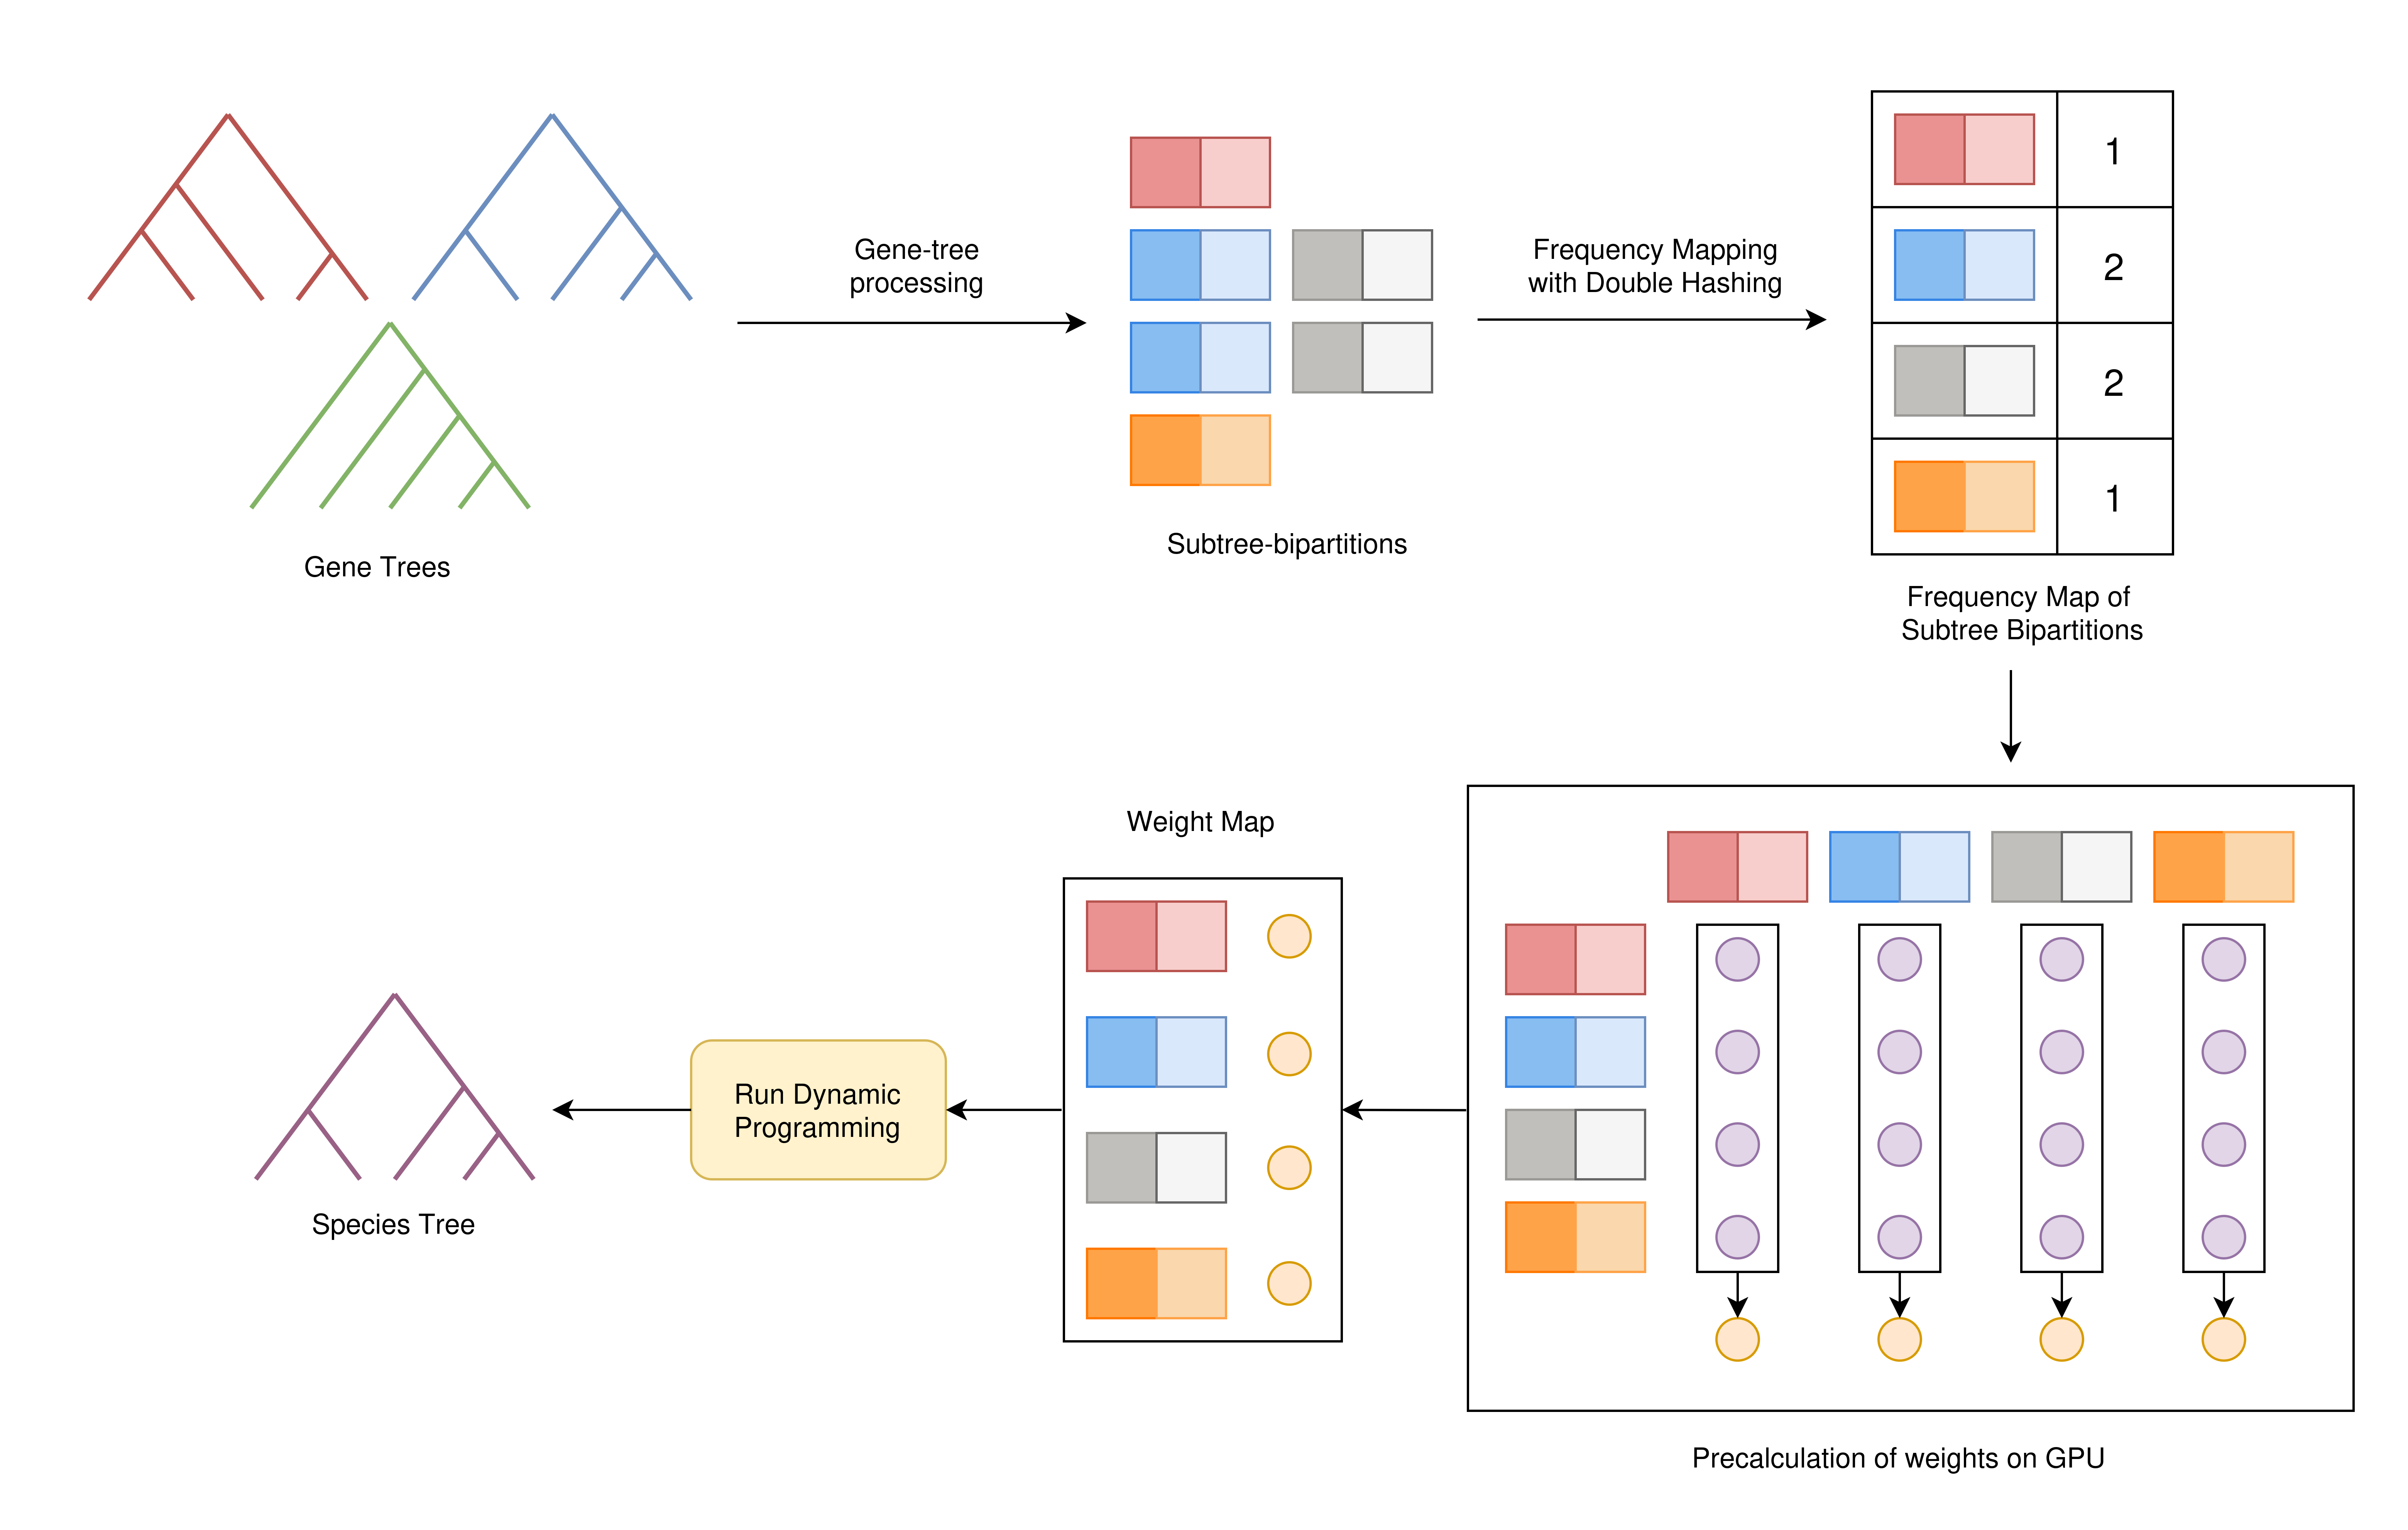
\includegraphics[width=0.9\linewidth]{fig-stx/v2-flow.png}
    \caption{Algorithmic Framework of STELAR-X Incorporating Dynamic Programming and GPU-Accelerated Weight Mapping}
    \label{fig:stelar-flow}
\end{figure}

\subsection{Formation of Candidate Subtree-Bipartitions}

\textcolor{blue}{TODO: need to write the inclusion of consensus trees and cite ASTRAL here, explaining why we may need extra bipartitions, and also saying in limitation and future work that consensus tree finding might itself present a bottleneck so finding wayaround for that...} 


\subsection{Frequency Mapping of Subtree Bipartitions using a compact representation (\addb{by mapping, we mean counting how many times a subtree-bipartition appears in the input gene trees?})}
\label{subsec:freq-mapping}

We consider the problem of calculating the frequency of each unique subtree-bipartition in $\mathcal{GB}$ across all gene trees in $\mathcal{G}$. A straightforward approach would be to run a bottom-up dynamic program that represents each subtree-bipartition as a bitset of length $n$ (the number of taxa). Using a Hashmap, these bitsets could then be counted to obtain a frequency mapping. However, this approach requires $O(n^{2}k)$ memory since there are $O(nk)$ total bipartitions, and each bitset requires $O(n)$ memory. This quadratic dependence on $n$ makes the method unsuitable for scaling to large numbers of taxa. We therefore propose an alternative representation of subtree-bipartitions that is both memory-efficient and computationally practical.

Consider a gene tree $g_i$, which can be expressed as the post-order traversal of its leaves, yielding a compact array representation $\mathcal{A}_i$. Let $u$ be an internal node in $g_i$ inducing the subtree-bipartition $(A|B)$. By construction, both $A$ and $B$ correspond to contiguous and adjacent subarrays of $\mathcal{A}_i$ because each bipartition corresponds to two contiguous and adjacent post-order intervals. Let $\mathcal{A}_{i,l,r}$ denote the subarray of $\mathcal{A}_i$ from indices $l$ to $r$. Then, if $A = \mathcal{A}_{i,l_1,r_1}$ and $B = \mathcal{A}_{i,l_2,r_2}$, the bipartition $(A|B)$ can be represented as the tuple $(i,l_1,r_1,l_2,r_2)$, where $l_1 < l_2$. In fact, since $l_2 = r_1 + 1$, four integers suffice to store the bipartition. This representation reduces the space requirement from $O(n^{2}k)$ to $O(nk)$.

We now focus on the efficient calculation of the frequency mapping under this representation. To do so, we first formalize the notion of equivalence between bipartitions. Let $P$ and $Q$ be sets of taxa. We write $P \sim Q$ if $P$ and $Q$ contain the same taxa, regardless of order. Two subtree-bipartitions $x = (A_1|B_1)$ and $y = (A_2|B_2)$ are said to be equivalent, denoted $x \equiv y$, if either $A_1 \sim A_2$ and $B_1 \sim B_2$, or $A_1 \sim B_2$ and $B_1 \sim A_2$. Thus, equivalence is invariant under permutation of taxa and under swapping of the bipartition sides.

Let $x = (i_x,l_{1x},r_{1x},l_{2x},r_{2x})$ and $y = (i_y,l_{1y},r_{1y},l_{2y},r_{2y})$ be two bipartitions. We distinguish two cases:
\begin{description}
    \item[Case 1: $i_x = i_y$.] Since both bipartitions arise from the same gene tree, their index ranges must either coincide exactly or be disjoint. In fact, two distinct bipartitions of the same tree cannot be equivalent. Therefore, $x \not\equiv y$.
    
    \item[Case 2: $i_x \neq i_y$.] When bipartitions originate from different gene trees, equivalence is possible. A naïve approach would compare the sets of taxa directly, requiring $O(n)$ time. To avoid this overhead, we employ a hashing-based technique that is both efficient and reliable.
\end{description}

We introduce a permutation-invariant and associative hash function $\phi$ that maps a set of taxa to a hash value independent of ordering. Associativity is essential, as it allows us to use prefix-scan arrays for efficient subarray hashing. Suppose $x \equiv y$. Then, by definition of equivalence, either 
\[
\mathcal{A}_{i_x,l_{1x},r_{1x}} \sim \mathcal{A}_{i_y,l_{1y},r_{1y}} \quad \text{and} \quad \mathcal{A}_{i_x,l_{2x},r_{2x}} \sim \mathcal{A}_{i_y,l_{2y},r_{2y}},
\]
or the same holds with the two sides swapped. Since $\phi$ is permutation-invariant, these relations imply
\[
\phi(\mathcal{A}_{i_x,l_{1x},r_{1x}}) = \phi(\mathcal{A}_{i_y,l_{1y},r_{1y}}) \quad \text{and} \quad \phi(\mathcal{A}_{i_x,l_{2x},r_{2x}}) = \phi(\mathcal{A}_{i_y,l_{2y},r_{2y}}),
\]
or the corresponding equalities under the swap. While equal hash values suggest possible equivalence, hash collisions prevent a strict guarantee. To make the probability of collisions negligible, we employ two safeguards.


% First, we adopt double hashing: we use two independent permutation-invariant hash functions, $\phi_1$ and $\phi_2$, and treat the pair $(\phi_1, \phi_2)$ as the final hash signature. Second, we apply an additional single-element hash function $\mathcal{H}$ to taxon identifiers before set-level hashing. Each taxon $t_j \in \mathcal{X}$ is assigned an identifier $d_j \in \{0,1,\ldots,n-1\}$, which is then mapped to a large integer $\mathcal{H}(d_j)$ in a sparse space. For a subarray $\mathcal{A}_{i,l,r}$, we compute
% \(
% \phi_1(\{\mathcal{H}(d_j)\}_{l \leq j \leq r}), \text{ and } \phi_2(\{\mathcal{H}(d_j)\}_{l \leq j \leq r})
% \) for the array $\mathcal{A}_i$.
% By leveraging associativity, we precompute prefix-scan arrays for $\phi_1$ and $\phi_2$, which allow subarray hash values to be computed in $O(1)$ time. All these calculations are performed within the finite field modulo a large prime $P$. Figure~\ref{fig:double-hashing} demonstrates an example of this approach.


First \addr{which one is second?}, we adopt double hashing: we use two independent permutation-invariant and associative hash functions, $\phi_1$ and $\phi_2$, and treat the pair $(\phi_1, \phi_2)$ as the final hash signature. Second, to further reduce the probability of hash collisions, we introduce an additional per-element hash function $\mathcal{H}$ that maps taxon identifiers to a sparse integer space before set-level hashing. Each taxon $t_j \in \mathcal{X}$ is assigned an identifier $d_j \in \{0,1,\ldots,n-1\}$, which is then transformed into a large integer $\mathcal{H}(d_j)$ modulo a prime field. This projection is essential because permutation-invariant hash functions such as SUM or XOR, when applied directly to small, contiguous identifiers, exhibit higher collision probabilities due to their limited combinatorial diversity. By first dispersing identifiers through $\mathcal{H}$, we ensure that the resulting hash space is sparse and the likelihood of accidental collisions is negligible. For a subarray $\mathcal{A}_{i,l,r}$, we compute
\[
\phi_1(\{\mathcal{H}(d_j)\}_{l \leq j \leq r}), \quad \text{and} \quad \phi_2(\{\mathcal{H}(d_j)\}_{l \leq j \leq r})
\]
for the array $\mathcal{A}_i$. Leveraging associativity, we precompute prefix-scan arrays for $\phi_1$ and $\phi_2$, enabling $O(1)$ computation of subarray hash values. All operations are performed within a finite field modulo a large prime $P$. Figure~\ref{fig:double-hashing} illustrates this approach.



% \begin{figure}
%     \centering
%     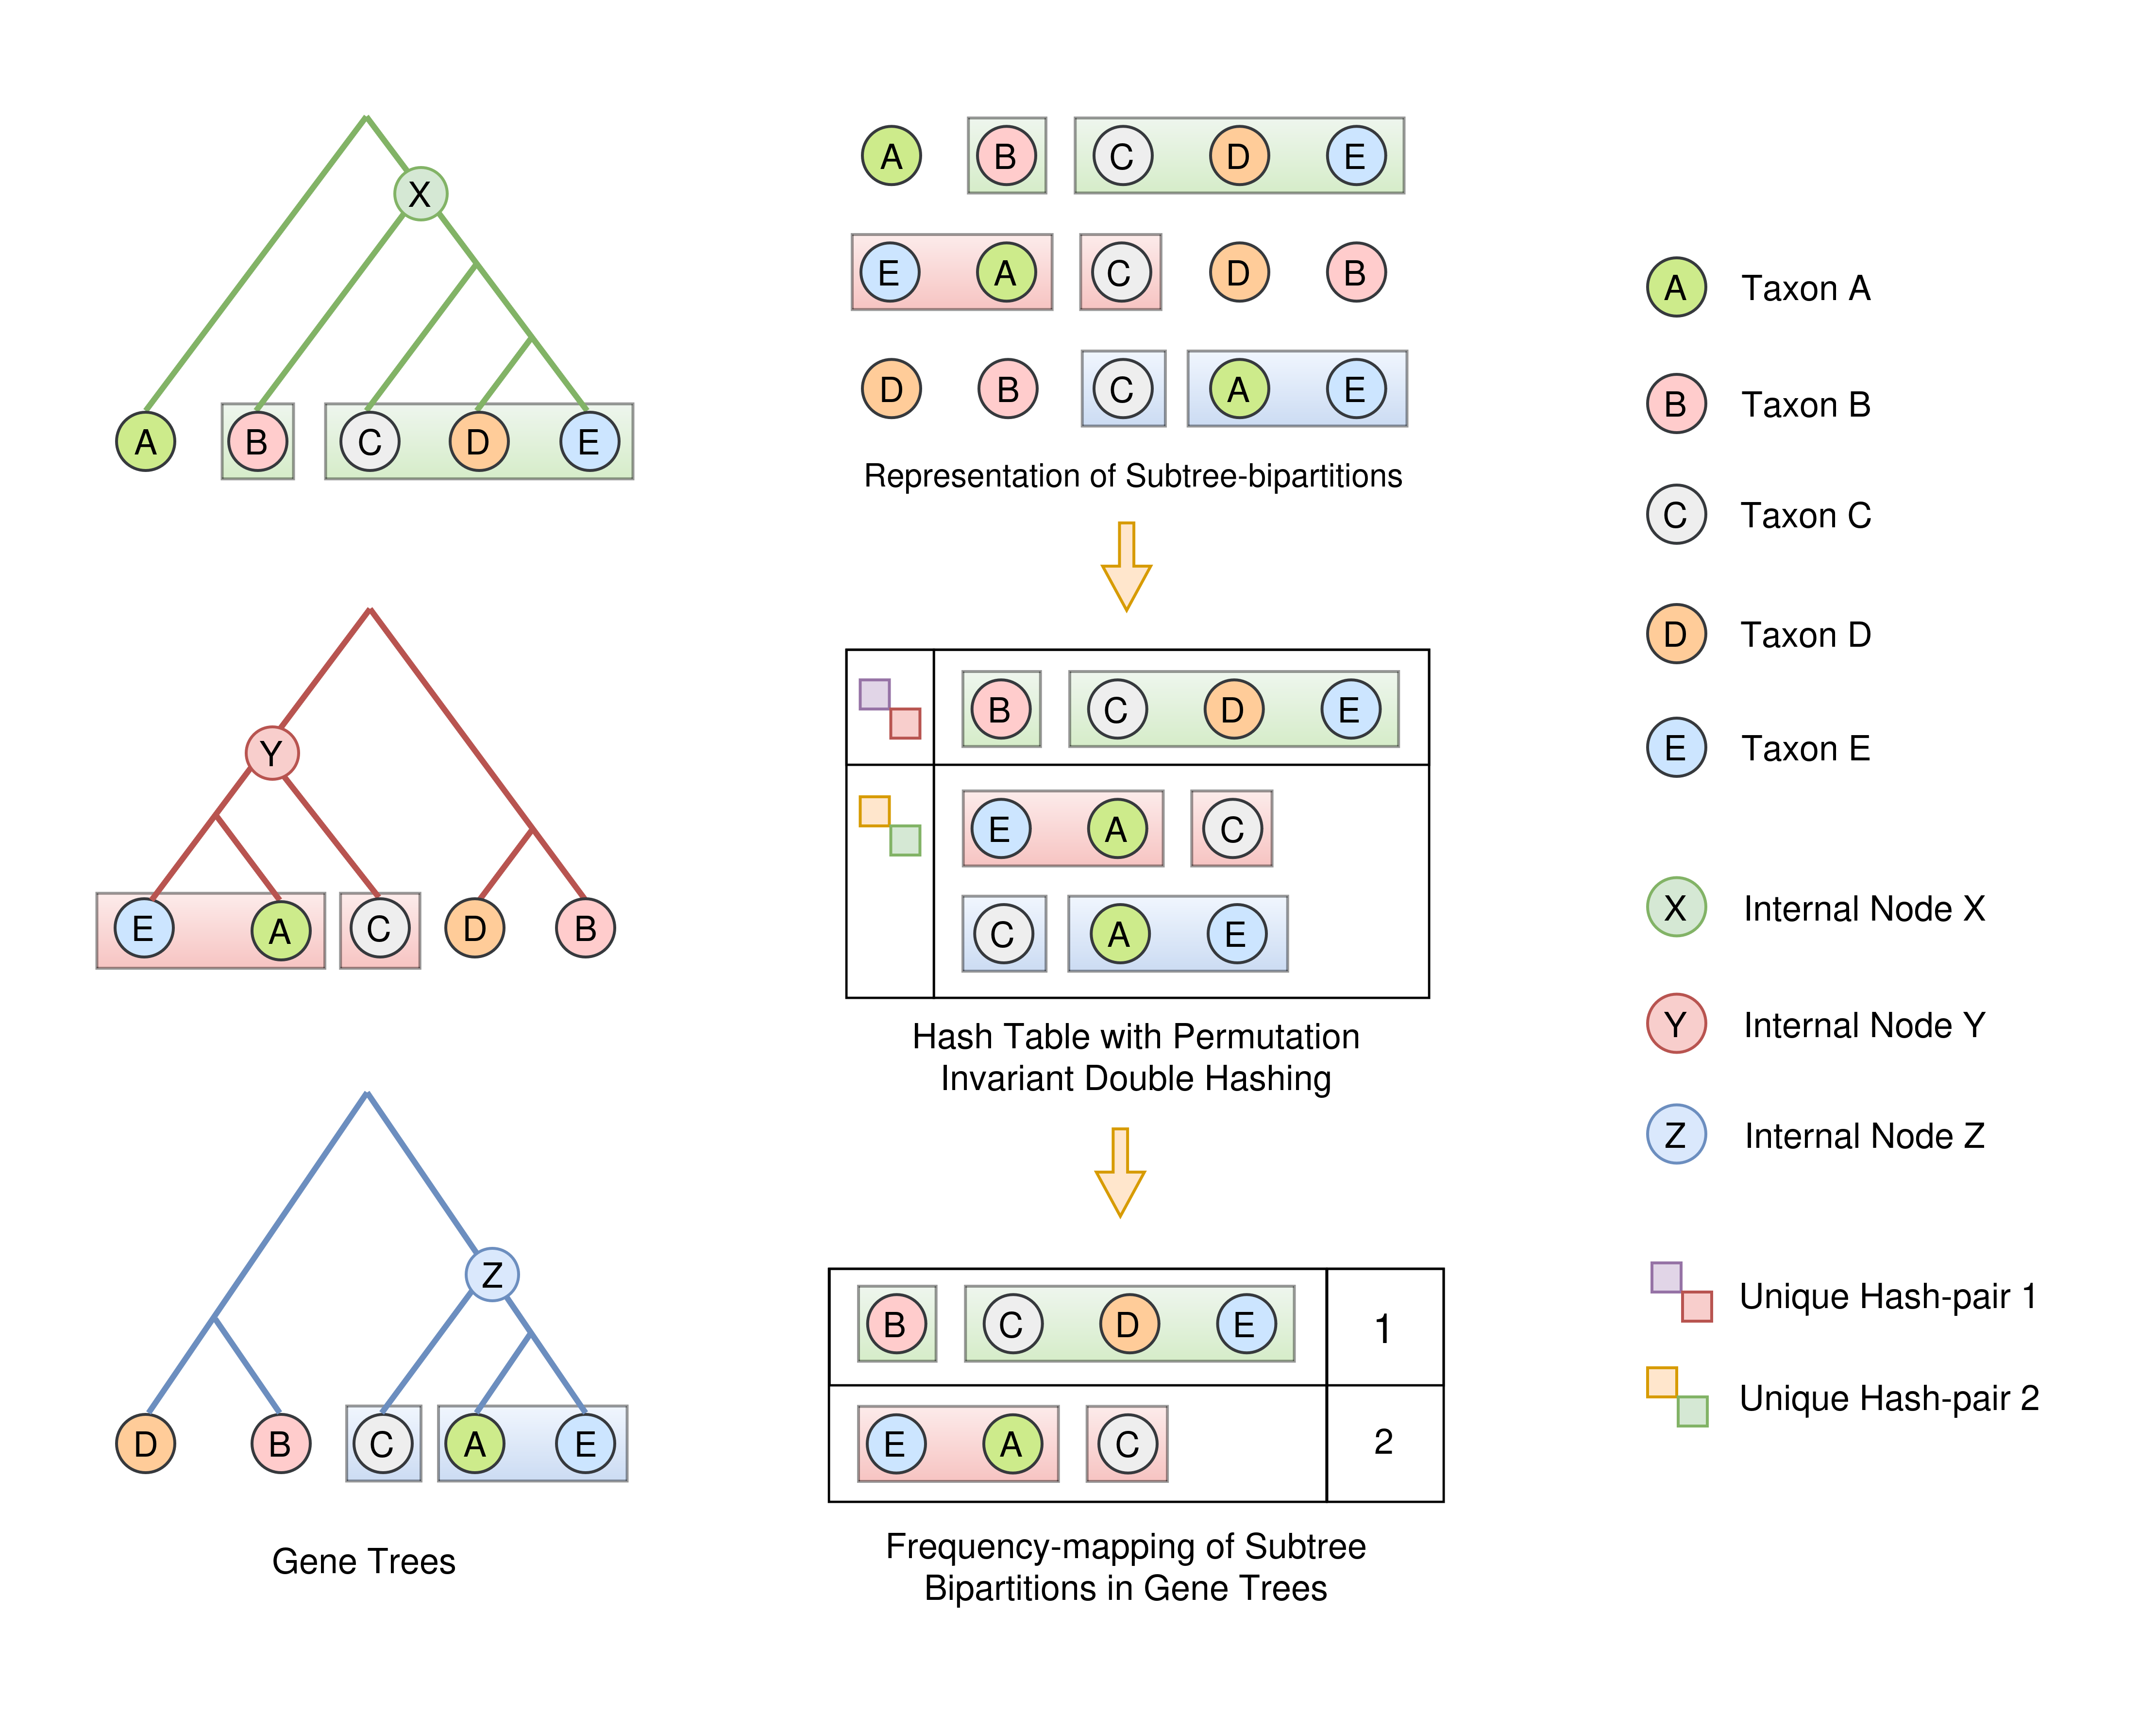
\includegraphics[width=0.9\linewidth]{fig-stx/v2-freq-mapping-double-hashing.png}
%     \caption{Example scenario of the frequency mapping of subtree-bipartitions with permutation-invariant double hashing. Three example subtree-bipartitions $(B|CDE)$, $(EA|C)$, and $(C|AE)$ are considered from the input gene trees. Since $(EA|C)$ and $(C|AE)$ are equivalent, they are mapped to the same hash-pair, enabling the subsequent determination of its frequency as 2.}
%     \label{fig:double-hashing}
% \end{figure}

\begin{figure}
    \centering
    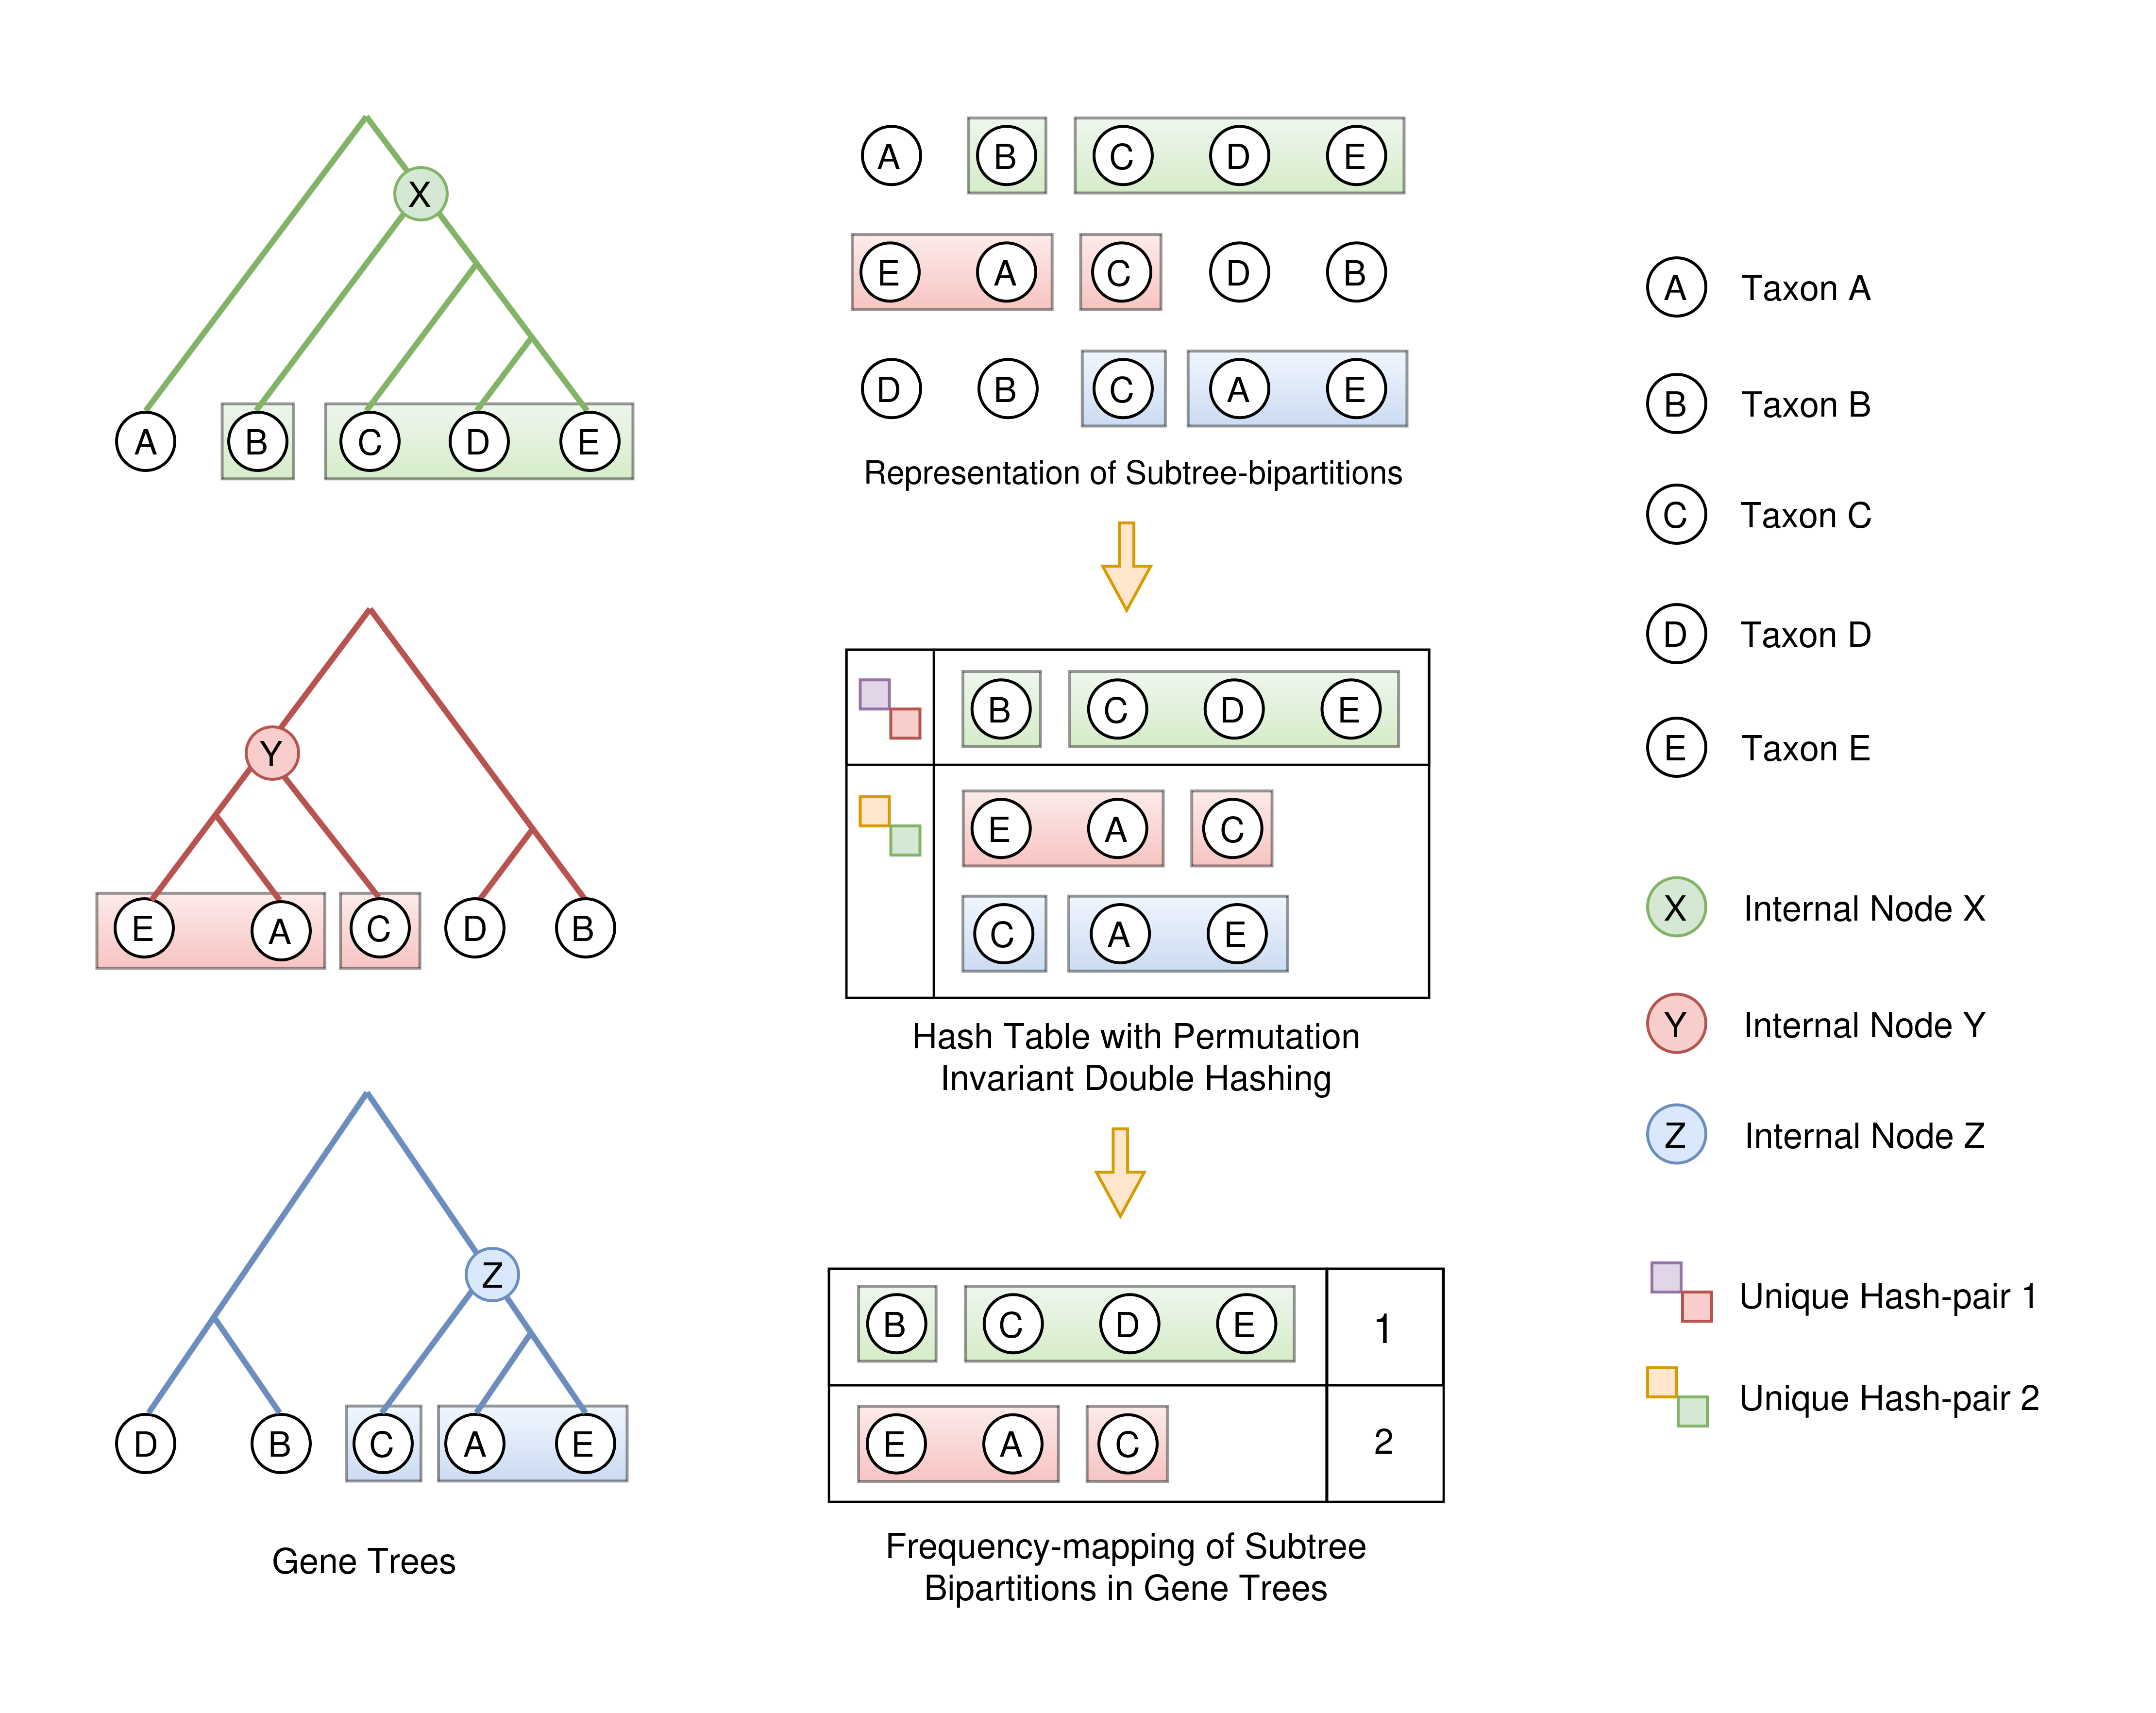
\includegraphics[width=0.9\linewidth]{fig-stx/v4-freq-mapping.png}
    \caption{Example scenario of the frequency mapping of subtree-bipartitions with permutation-invariant double hashing. Three example subtree-bipartitions $(B|CDE)$, $(EA|C)$, and $(C|AE)$ are considered from the input gene trees. Since $(EA|C)$ and $(C|AE)$ are equivalent, they are mapped to the same hash-pair, enabling the subsequent determination of its frequency as 2.}
    \label{fig:double-hashing}
\end{figure}

In practice, this combination of double hashing and sparse integer mapping makes collisions vanishingly rare. In our implementation, we employ the SUM function as $\phi_1$ and the XOR function as $\phi_2$. Across extensive experiments with large datasets, we did not encounter a single collision, demonstrating the robustness of the proposed method.

Finally, we use the hash table to construct a frequency mapping of the unique subtree-biparititions in $O(\mathcal{|GB|})$ time.








\paragraph{Theoretical Analysis of Collision Probability}  

Now we provide a theoretical analysis of the probability of collisions. The key intuition is that collisions are rare because whenever two sets differ, at least one taxon contributes an independent random value, making accidental equality highly unlikely.

Let $\mathcal{X}$ be the taxon set with $|\mathcal{X}|=n$. Let $M$ be the number of subtree-bipartitions produced across all gene trees (in our setting, $M=\Theta(nk)$). We choose a large prime $P$ and work in the field $\mathbb{F}_P$.

\textbf{Setup.} A single-element hash
\[
\mathcal{H}:\{0,\dots,n-1\}\to\mathbb{F}_P
\]
maps each taxon identifier $d_j$ to
\[
r_j \coloneqq \mathcal{H}(d_j)\in\mathbb{F}_P.
\]
We idealize that the values $\{r_j\}_{j=1}^n$ are independent and uniformly distributed in $\mathbb{F}_P$.

We then apply two associative, permutation-invariant set-level functions $\phi_1,\phi_2$, each operating directly on subsets of $\{r_j\}$. The signature of a set $S$ is
\[
\sigma(S) \coloneqq \big(\phi_1(\{r_j:j\in S\}),\, \phi_2(\{r_j:j\in S\})\big).
\]

\textbf{Single-set collision probability.}  
Let $S\neq T$ and define $U=S\setminus T$, $V=T\setminus S$. Associativity ensures that $\phi_a$ admits a natural cancellation operator $\ominus$ (e.g. subtraction for addition, XOR for XOR, etc.), so that
\[
\phi_a(S)\ominus\phi_a(T) \;=\; \phi_a(U)\ominus\phi_a(V).
\]
Because $U\cup V\neq\varnothing$, at least one $r_t$ appears only in one side. Conditioning on all other $r_j$, the difference reduces to a function of the uniform random variable $r_t$. This equals zero with probability at most $1/P$. Thus
\begin{equation}\label{eq:single-hash}
\Pr\big(\phi_a(S)=\phi_a(T)\big) = \frac{1}{P}.
\end{equation}

\textbf{Pairwise signature collision.}  
Suppose the two set-level functions $\phi_1$ and $\phi_2$ are constructed so that their collision events are statistically independent (e.g.\ by using independent salts or structurally distinct definitions of $\phi_a$). Then for distinct sets $S,T$,
\[
\Pr\big(\sigma(S)=\sigma(T)\big)
= \Pr\big(\phi_1(S)=\phi_1(T)\big)\cdot \Pr\big(\phi_2(S)=\phi_2(T)\big)
= \frac{1}{P^2}.
\]



\textbf{Collision probability for bipartitions.}  
Let bipartitions $x=(A_1 \mid B_1)$ and $y=(A_2 \mid B_2)$ be distinct (non-equivalent).  
A collision occurs if and only if
\[
\big(\sigma(A_1)=\sigma(A_2)\ \wedge\ \sigma(B_1)=\sigma(B_2)\big)
\quad\text{or}\quad
\big(\sigma(A_1)=\sigma(B_2)\ \wedge\ \sigma(B_1)=\sigma(A_2)\big).
\]
Since each matching holds with probability $1/P^2$, we obtain
\[
\Pr\!\big(\text{collision between }x\text{ and }y\big) \;\le\; \frac{2}{P^2}.
\]




\textbf{Global (any-pair) collision probability.}  
Among $M$ bipartitions there are at most $\binom{M}{2}$ pairs. By a union bound,
\[
\Pr(\exists\ \text{collision}) \;\le\; \binom{M}{2}\cdot \frac{2}{P^2}
\;\le\; \frac{M^2}{P^2}.
\]
To keep this probability below a prescribed tolerance $\delta$, it suffices to ensure that
\[
P \;\geq\; \frac{M}{\sqrt{\delta}}.
\]
Hence, choosing $P$ sufficiently larger than $M$ renders global collisions negligible in practice.






\subsection{Precomputation of Bipartition Weights}
\label{subsec:weight-precomp}

We now turn to the theoretical justification for the precomputation of weights associated with all candidate bipartitions in $\mathcal{CB}$. We first explain why these weights are necessary for the dynamic programming (DP) algorithm of STELAR, and then argue that, under the constrained setting, all subtree-bipartitions in $\mathcal{GB}$ must eventually be explored.

Recall that the recursive formulation of STELAR (Equation~\eqref{eq:recurrence-relation}) defines the state space of the DP algorithm. Figure~\ref{fig:stelar-dp} provides an illustration of this state space. Intuitively, the DP begins with a cluster containing all taxa in $\mathcal{X}$. From this initial state, transitions are governed by subtree-bipartitions that partition the taxa of the current cluster. Thus, the evolution of the state space directly depends on the collection of bipartitions available. We now show that, in the constrained version of STELAR, this process inevitably requires the weights of all subtree-bipartitions in $\mathcal{GB}$.

\begin{theorem}
    \label{th:dp-span}
    If $\mathcal{CB} = \mathcal{GB}$, then the state space of the DP algorithm spans every subtree-bipartition $x \in \mathcal{CB}$.
\end{theorem}

\begin{proof}
    We argue by contradiction. Suppose there exists a bipartition $x = (A|B) \in \mathcal{CB}$ that is not explored in the state space of the DP. We consider two possible cases:

    \begin{description}
        \item[Case 1: $A \cup B = \mathcal{X}$]  
        Since $\mathcal{CB} = \mathcal{GB}$, we have $x \in \mathcal{GB}$. As $A \cup B$ covers all taxa, $x$ corresponds to a root-level bipartition in one of the gene trees. By construction, such bipartitions are included in the search space at the very first state transition. This contradicts our assumption that $x$ is not explored.

        \item[Case 2: $A \cup B \neq \mathcal{X}$]  
        Again, $x \in \mathcal{GB}$ and hence arises from some internal node $u$ of a gene tree $g_i$, where the taxa covered by $u$ form the set $\mathcal{Y} = A \cup B$. Since $\mathcal{Y} \subsetneq \mathcal{X}$, $u$ must have a parent node $p$ in $g_i$. Let the bipartition induced by $p$ be $y = (C|D)$. By construction, either $C = \mathcal{Y}$ or $D = \mathcal{Y}$. Thus, if $y$ is explored in the DP state space, then the algorithm must also explore its child bipartition $x$, by design of the transition rules. Hence, the assumption that $x$ is not explored implies that $y$ is also not explored. Repeating this reasoning along the ancestor chain of $u$, we eventually reach the root of $g_i$, where Case~1 applies and yields a contradiction.
    \end{description}

    Since both cases lead to contradictions, our assumption is false. Therefore, every subtree-bipartition $x \in \mathcal{GB}$ is necessarily explored in the constrained DP state space. Thus, precomputing weights is reasonable and justifies isolating this step for GPU acceleration.
\end{proof}

This result shows that, in the constrained setting where $\mathcal{CB} = \mathcal{GB}$, the dynamic programming algorithm must access the weights of all bipartitions in $\mathcal{GB}$. Furthermore, even when $\mathcal{GB} \subsetneq \mathcal{CB}$, as long as $|\mathcal{CB}|$ is not asymptotically larger than $|\mathcal{GB}|$, it remains practical to precompute the weights of all subtree-bipartitions in $\mathcal{CB}$.


We now describe our strategy for precomputing the weights of candidate bipartitions. We begin by recalling the formulation for computing the weight of a single bipartition. Let $x = (A_1|B_1) \in \mathcal{CB}$ denote a candidate subtree-bipartition, and let $y = (A_2|B_2) \in \mathcal{SBP}(g_i)$ be a bipartition in a gene tree $g_i$. It was shown in \cite{stelar} that the number of triplets simultaneously mapped to both $x$ and $y$ can be expressed as

\begin{equation}
\mathcal{M}(x,y) = \mathcal{NT}(|A_{1} \cap A_{2}|, |B_{1} \cap B_{2}|) 
+ \mathcal{NT}(|A_{1} \cap B_{2}|, |A_{2} \cap B_{1}|),
\label{eq:Mxy}
\end{equation}

where $\mathcal{NT}(n_1,n_2)$ denotes the total number of triplets mapped to a subtree-bipartition $(A|B)$ of a rooted binary tree, with $|A| = n_1$ and $|B| = n_2$. A straightforward combinatorial argument yields,

\begin{equation}
\mathcal{NT}(n_1, n_2) = \binom{n_1}{2}\binom{n_2}{1} + \binom{n_2}{2}\binom{n_1}{1} 
= \frac{n_1 n_2 (n_1 + n_2 - 2)}{2}.
\label{eq:NT}
\end{equation}

Using these definitions, the weight of bipartition $x$ with respect to the set of gene trees $\mathcal{G}$ can be written as

\begin{equation}
w_{\mathcal{G}}(x) = \sum_{i=1}^{k} \; \sum_{y \in \mathcal{SBP}(g_i)} \mathcal{M}(x,y).
\end{equation}

To reduce computational cost, we take advantage of the frequency mapping of unique subtree-bipartitions obtained earlier. Specifically, let $f_{\mathcal{G}}(y)$ denote the frequency of bipartition $y \in \mathcal{GB}$ across all gene trees in $\mathcal{G}$. Then the weight of $x$ can be equivalently expressed as,

\begin{equation}
w_{\mathcal{G}}(x) = \sum_{y \in \mathcal{GB}} f_{\mathcal{G}}(y)\,\mathcal{M}(x,y).
\label{eq:effcal}
\end{equation}


Equations~\eqref{eq:Mxy} and \eqref{eq:NT} together imply that the finding $\mathcal{M}(x,y)$ requires efficient computation of intersection counts between clusters of taxa. If we convert the unique subtree-bipartitions into bitsets for intersection counting, they would again increase the memory consumption. We, therefore, proceed with the same integer tuple representation of subtree-biparititons. We now describe the method of finding intersection counts efficiently using this representation. 

Let $X = \mathcal{A}_{i,l_{x},r_{x}}$ and $Y = \mathcal{A}_{j,l_{y},r_{y}}$ denote two clusters of taxa where $i \neq j$. We want to find $|X \cap Y|$. It is easy to see that, $|X| = r_x - l_x+1$ and $|Y| = r_y - l_y+1$. We thus first find the cluster having the smaller number of taxa. Without loss of generality, let $|X| < |Y|$. We now iterate over the taxa in this smaller cluster $X$ and for each taxon we find whether this taxon belongs to the cluster $Y$. To optimize this membership testing, we precompute an index map $\pi_i$ for each gene tree $g_i$, mapping a taxon $v \in \mathcal{X}$ to its position in the array representation $\mathcal{A}_i$. Therefore, 

\[
\pi_i(v) = \text{position of } v \text{ in } \mathcal{A}_i
\]

Thus, for each taxon $v \in \mathcal{A}_{i,l_{x},r_{x}}$, we check whether $l_y \leq \pi_j(v) \leq r_y$ and accumulate the intersection count thereby in $O(\text{min}(|X|,|Y|)$ time. We now present a theoretical bound on the running time of this precomputation over all the bipartitions under balanced gene-tree assumption.




\begin{theorem}
\label{th:precompute-bound}
Assume $\mathcal{CB} = \mathcal{GB}$, where $\mathcal{GB}$ contains all subtree bipartitions across the $k$ gene trees. In other words, every bipartition across all gene trees is unique. If each gene tree is a perfectly balanced rooted binary tree with $n = 2^{d}$ taxa, then the precomputation of weights requires $\mathcal{O}(n^{2}k^{2})$ time.

\end{theorem}

\begin{proof}
By Equation~\eqref{eq:effcal}, computing the weight of each candidate
bipartition requires evaluating \(\mathcal{M}(x,y)\) against every
\(y\in\mathcal{GB}\). Thus we must evaluate \(\mathcal{M}(x,y)\) for
every ordered pair \((x,y)\in\mathcal{GB}\times\mathcal{GB}\). We bound
the total cost by first bounding the cost between two fixed balanced
trees and then summing over the tree-pairs.

In a perfectly balanced rooted binary tree on \(n=2^{d}\) leaves,
an internal node at depth \(\ell\) (root at depth \(0\)) has subtree
size \(n/2^{\ell}\), and each of its two child subtrees has size
\(s = n/2^{\ell+1}\). Thus the set of possible child-subtree sizes is
\[
\mathcal{S}=\{\,2^{0},2^{1},\dots,2^{d-1}\,\},
\]
and for a given child-subtree size \(s\in\mathcal{S}\) the number of
internal nodes whose child-subtrees have size \(s\) equals the number of
disjoint blocks of size \(2s\) that partition the \(n\) leaves, i.e.
\(\frac{n}{2s}\). Therefore the number of subtree-bipartitions in one balanced tree whose parts (child-subtrees) have size \(s\)
is \(n/(2s)\).

\textbf{Per-pair cost in terms of sizes.}
We consider two bipartitions \(x=(A_{1}|B_{1})\) in tree \(g_p\) and
\(y=(A_{2}|B_{2})\) in tree \(g_q\), and let the child-subtree sizes
be \(s\) and \(t\), respectively. So \(|A_{1}|=|B_{1}|=s\) and
\(|A_{2}|=|B_{2}|=t\)). By Equation~\eqref{eq:Mxy}, \(\mathcal{M}(x,y)\)
depends on four intersection counts among the parts of \(x\) and
\(y\). Each such intersection can be computed by iterating over the
smaller argument using the index map \(\pi\), hence the time to compute each intersection is \(O(\min(s,t))\). Since there are only a constant number of
such intersections, the total cost to evaluate \(\mathcal{M}(x,y)\) is
\[
\operatorname{cost}(\mathcal{M}(x,y)) \;=\; O(\min(s,t)).
\]

\textbf{Cost between two balanced trees.}
We now group bipartitions of \(g_p\) and \(g_q\) by their child-subtree sizes
\(s=2^{i}\) and \(t=2^{j}\) (with \(0\le i,j\le d-1\)). The number of
bipartitions in \(g_p\) with part-size \(s\) is \(n/(2s)\), and similarly
for \(g_q\) with part-size \(t\). Thus the number of ordered bipartition
pairs with sizes \((s,t)\) is \(\frac{n}{2s}\cdot\frac{n}{2t}\), and the
contribution of this size-class pair to the cost is
\[
\frac{n}{2s}\cdot\frac{n}{2t}\cdot O(\min(s,t))
= O\!\left(\frac{n^{2}\min(s,t)}{4st}\right)
= O\!\left(\frac{n^{2}}{4\max(s,t)}\right).
\]
Replacing \(s=2^{i}\) and \(t=2^{j}\), the total cost between the two
trees is
\[
S_{pq} \;=\; O\!\left(n^{2}\sum_{i=0}^{d-1}\sum_{j=0}^{d-1} 2^{-\max(i,j)}\right).
\]


We evaluate the double sum by symmetry. Splitting the domain into the two
triangles \(i\le j\) and \(i>j\):
\begin{align*}
\sum_{i=0}^{d-1}\sum_{j=0}^{d-1}2^{-\max(i,j)}
&=\sum_{j=0}^{d-1}\sum_{i=0}^{j}2^{-j}
  +\sum_{i=0}^{d-1}\sum_{j=0}^{i-1}2^{-i} \\[4pt]
&=\sum_{j=0}^{d-1}(j+1)2^{-j}
  +\sum_{i=0}^{d-1}i\,2^{-i} \\[4pt]
&=2\sum_{k=0}^{d-1}\frac{k}{2^{k}}
  +\sum_{k=0}^{d-1}\frac{1}{2^{k}}.
\end{align*}
Both finite sums are uniformly bounded as \(d\) grows, since
\(\sum_{k\ge0}k/2^{k}=2\) and \(\sum_{k\ge0}1/2^{k}=2\).
Hence
\[
\sum_{i=0}^{d-1}\sum_{j=0}^{d-1}2^{-\max(i,j)} \le 6,
\]
and in fact the exact value is
\[
\sum_{i=0}^{d-1}\sum_{j=0}^{d-1}2^{-\max(i,j)}
=6-\frac{2d+3}{2^{\,d-1}}.
\]
Therefore the double sum is \(O(1)\).




Hence \(S_{pq}=O(n^{2})\). Thus, computing all pairwise
intersection costs between bipartitions of two balanced trees costs
\(O(n^{2})\).

\textbf{Extension to $k$ trees.}
There are \(k\) gene trees and thus \(k^{2}\) ordered pairs of trees.
Summing the \(O(n^{2})\) cost over all ordered pairs yields the
total precomputation cost
\(O(n^{2})\cdot k^{2}=O(n^{2}k^{2})\), which proves the theorem.
\end{proof}

Our analysis assumes perfectly balanced binary trees for mathematical tractability. However, because the runtime for each bipartition pair primarily depends on the minimum of the corresponding subtree sizes, the overall running time is expected to remain close to the derived asymptotic bound in realistic scenarios. Only in extreme cases where most gene trees are highly unbalanced would we incur notable deviations. In practice, such imbalance is further mitigated by the fact that the number of unique bipartitions, $|\mathcal{GB}|$, is generally smaller than $nk$. Hence, the balanced-tree assumption provides a reasonable approximation of empirical behavior.

\subsection{Execution of Dynamic Programming}
\label{subsec:dp}

As the final step of our algorithm, we execute the dynamic programming procedure using the recursive relation defined in Equation~\eqref{eq:recurrence-relation}. During this execution, an essential requirement is to efficiently identify all subtree-bipartitions $x \in \mathcal{CB}$ that partition the cluster corresponding to the current state.  

To address this, we precompute a map that explicitly defines the state space. Let $x = (A|B) \in \mathcal{CB}$ be a candidate subtree-bipartition. By construction, $x$ partitions the cluster formed by the taxa set $C = A \cup B$. Accordingly, we define a mapping

\[
\Psi : \{\text{clusters of taxa}\} \;\longrightarrow\; \mathcal{CB},
\qquad 
% \Phi(A \cup B) = \{\, x = (A|B) \,\}.
\Psi(C) = \{\, x = (A|B) \in \mathcal{CB} \mid A \cup B = C \,\},
\]

% Here we have updated the new approach

For each subtree-bipartition $x = (A|B) \in \mathcal{CB}$, we record its associated cluster $C = A \cup B$, thereby establishing a direct correspondence between each candidate bipartition and the cluster it partitions. At this stage, we again employ the double hashing technique to encode these clusters in the state space, thereby avoiding the use of memory-intensive bitset representations. Specifically, for each cluster $C$, we compute a pair of hash signatures $(\phi_1(C), \phi_2(C))$, which uniquely identifies the cluster and maps it to its corresponding subtree-bipartitions. The algorithm then utilizes this precomputed state-space map, together with the weight map described earlier, to efficiently execute the dynamic programming recurrence. The overall workflow of this procedure is illustrated in Figure~\ref{fig:stelar-dp}.




\begin{figure}
    \centering
    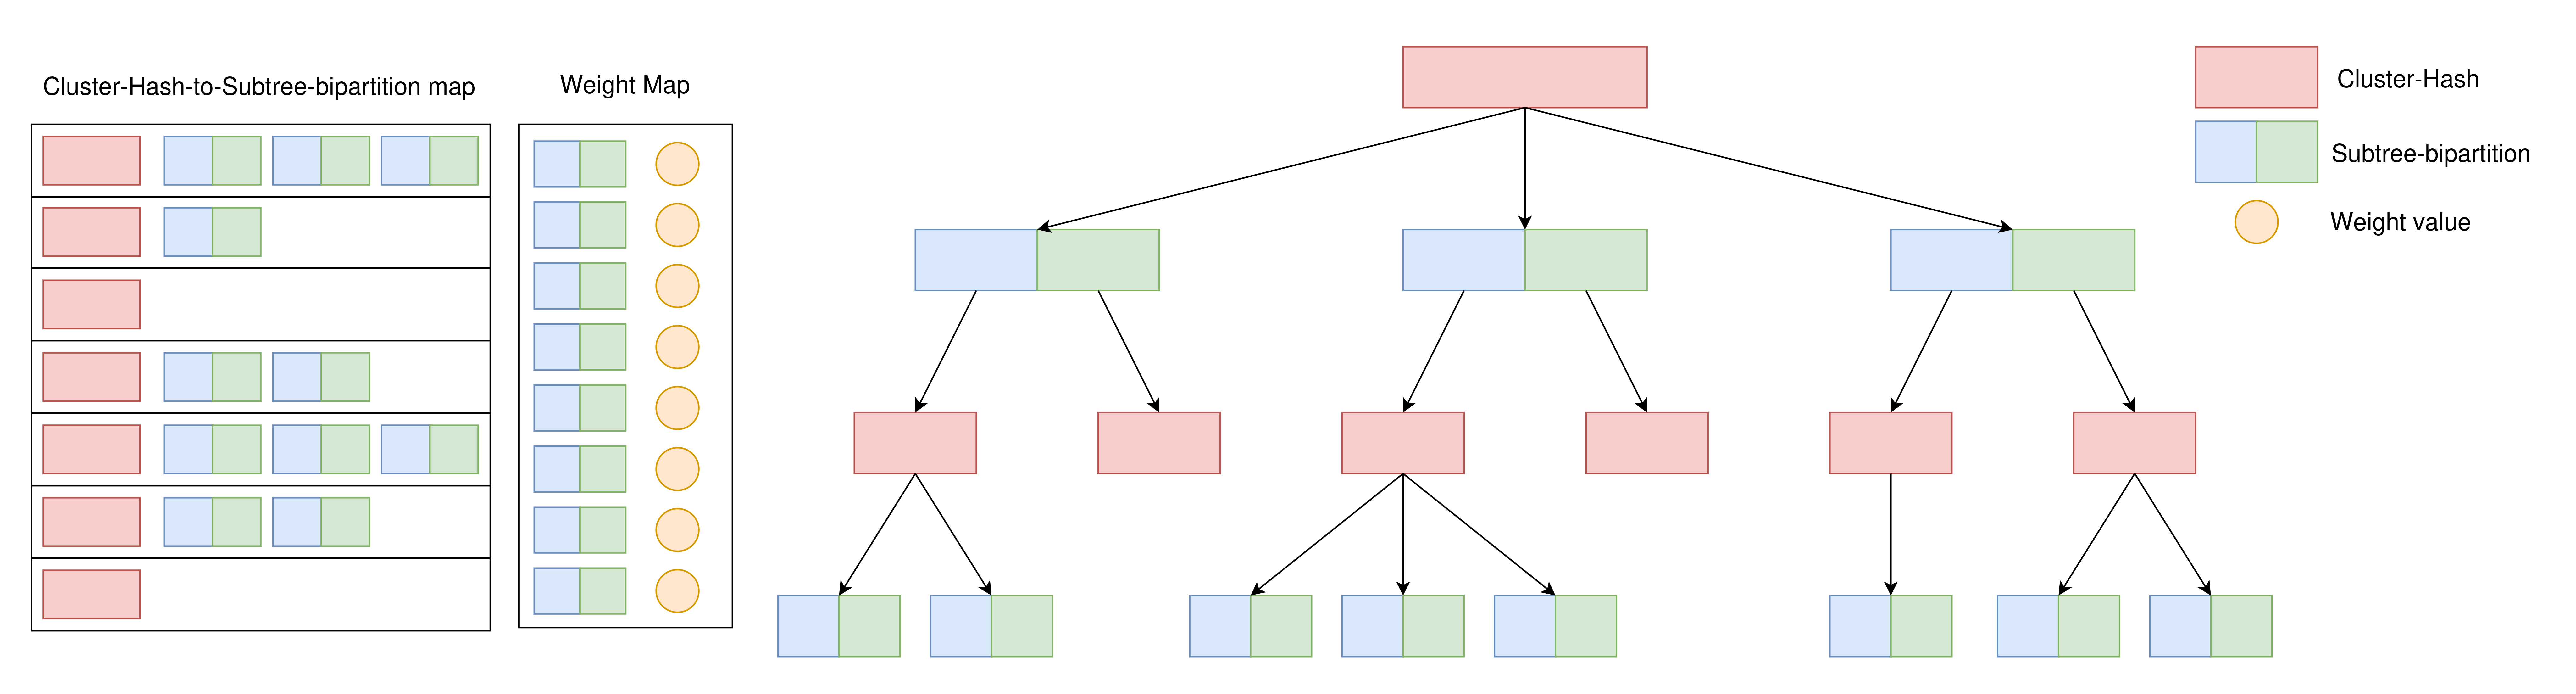
\includegraphics[width=0.98\linewidth]{fig-stx/v3-dp-alg.png}
    \caption{Dynamic programming algorithm in STELAR-X using cluster-hash to subtree-bipartition map and precomputed weight map}
    \label{fig:stelar-dp}
\end{figure}

\subsection{Parallelization}
\label{subsec:parallel}

We next identify the stages of our algorithm that are amenable to CPU and GPU parallelization. For the complexity analysis, we assume the availability of $T_\mathcal{C}$ CPU threads and $T_\mathcal{G}$ GPU threads that can be executed concurrently. These quantities represent the degree of parallelism achievable under the ideal assumption of perfect load balancing and negligible synchronization or communication overhead. In practice, the actual speedup may be lower; however, this assumption provides a standard theoretical framework for expressing parallel time complexity. 


\subsubsection{CPU Parallelization}

We primarily employ CPU parallelization for parsing and processing the $k$ gene trees. Specifically, the set of gene trees is partitioned into $T_\mathcal{C}$ chunks of approximately equal size, and each chunk is processed in parallel by a separate thread. During the processing of each gene tree, the corresponding frequency mapping is also computed within the same thread. When necessary, thread-safe data structures and synchronization mechanisms are employed to ensure the correct accumulation of values across threads.


\subsubsection{GPU Parallelization}

We employ GPU acceleration for the precomputation of bipartition weights. As derived earlier, the weight of a single bipartition can be obtained by finding intersection counts across bipartitions using the integer tuple representation. To compute the weights for all candidate bipartitions $x \in \mathcal{CB}$, it is therefore necessary to evaluate $\mathcal{M}(x,y)$ for every pair $(x,y)$ where $x \in \mathcal{CB}$ and $y \in \mathcal{GB}$. This corresponds to executing the same operation across $O(|\mathcal{CB}||\mathcal{GB}|)$ bipartition pairs, followed by accumulation along the $\mathcal{GB}$ dimension to obtain the weights of $O(|\mathcal{CB}|)$ candidate bipartitions.  

We leverage this highly regular computation pattern to parallelize the precomputation over $T_\mathcal{G}$ GPU threads. In practice, all bipartitions $x \in \mathcal{CB}$ and $y \in \mathcal{GB}$ are encoded as integer tuples and transferred to GPU memory. In addition, the in-order traversal arrays and the index maps are also transferred to GPU. The results are then aggregated to produce a weight map containing $O(|\mathcal{CB}|)$ entries, which directly feeds into the dynamic programming algorithm. Additional low-level optimizations, such as efficient memory sharing and tiling, are employed to reduce memory latency and further improve throughput.


\subsection{Complexity Analysis}
\label{subsec:complexity}

We now provide a theoretical analysis of the running time and memory requirement of STELAR-X. 

\subsubsection{Running Time Analysis}

The parsing of the $k$ input trees over $T_\mathcal{C}$ CPU threads requires $O\!\left(\tfrac{nk}{T_\mathcal{C}}\right)$ time. The subsequent computation of the frequency mapping, using the double-hashing approach, also requires $O\!\left(\tfrac{nk}{T_\mathcal{C}}\right)$ time. This efficiency follows from the use of prefix-scan arrays, which enable constant-time range hash evaluations. Next, the precomputation of weights, distributed across $T_\mathcal{G}$ GPU threads, requires $O\!\left(\tfrac{n^2k^2}{T_\mathcal{G}}\right)$ time under the balanced gene tree assumption as derived earlier. 

Finally, we analyze the running time of the dynamic programming (DP) algorithm. By Equation~\eqref{eq:recurrence-relation} and Theorem~\ref{th:dp-span}, the size of the DP state space is at most $O(|\mathcal{CB}|)$. Since both the state-space map and the weight map are precomputed, the DP algorithm itself executes in $O(|\mathcal{CB}|)$ time.  

Putting all components together, the total running time of our algorithm under the balanced tree assumption is
\[
O\!\left(
\tfrac{nk}{T_\mathcal{C}} \;+\;
\tfrac{n^2k^2}{T_\mathcal{G}} \;+\;
|\mathcal{CB}|
\right).
\]


\subsubsection{Memory Analysis} 

We now analyze the memory requirements of our algorithm in both CPU RAM and GPU VRAM.  

On the CPU side, storing the $k$ input gene trees over $n$ taxa requires $O(nk)$ memory. The efficient representation of subtree-bipartitions, together with their subsequent processing, also requires $O(nk)$ memory. Storing the unique subtree bipartitions in $\mathcal{GB}$ and $\mathcal{CB}$ requires $O(|\mathcal{GB}|+|\mathcal{CB}|)$ space. The dynamic programming algorithm requires $O(|\mathcal{CB}|)$ additional space. Overall, the total CPU memory usage is therefore
\[
O\!\left(nk + |\mathcal{GB}| + |\mathcal{CB}|\right).
\]

On the GPU side, memory usage is dominated by the precomputation of weights. Each bipartition is represented as a constant-length integer tuple. Consequently, the total GPU VRAM required for storing all $O(|\mathcal{GB}|+|\mathcal{CB}|)$ bipartitions is 
\[
O\!\left(|\mathcal{GB}|+|\mathcal{CB}|)\right.
\]

Since both $|\mathcal{GB}|$ and $|\mathcal{CB}|$ can be bounded by $O(nk)$, the overall CPU and GPU memory consumption scales as $O(nk)$, matching the asymptotic input-space complexity.



\section{Results}

\subsection{Experimental Setup}

All experiments were conducted on a server equipped with an NVIDIA RTX 4090 GPU (24 GB VRAM) and an AMD EPYC 7742 CPU with 32 active cores and 129 GB RAM.

\subsubsection{Datasets}

\textcolor{blue}{TODO: simulated - simulation parameters, biological - 1kp, avian}

\subsubsection{Experimental Environment}


\subsection{Accuracy of Inference}

\textcolor{blue}{TODO: descriptions of results}

\begin{figure}
    \centering
    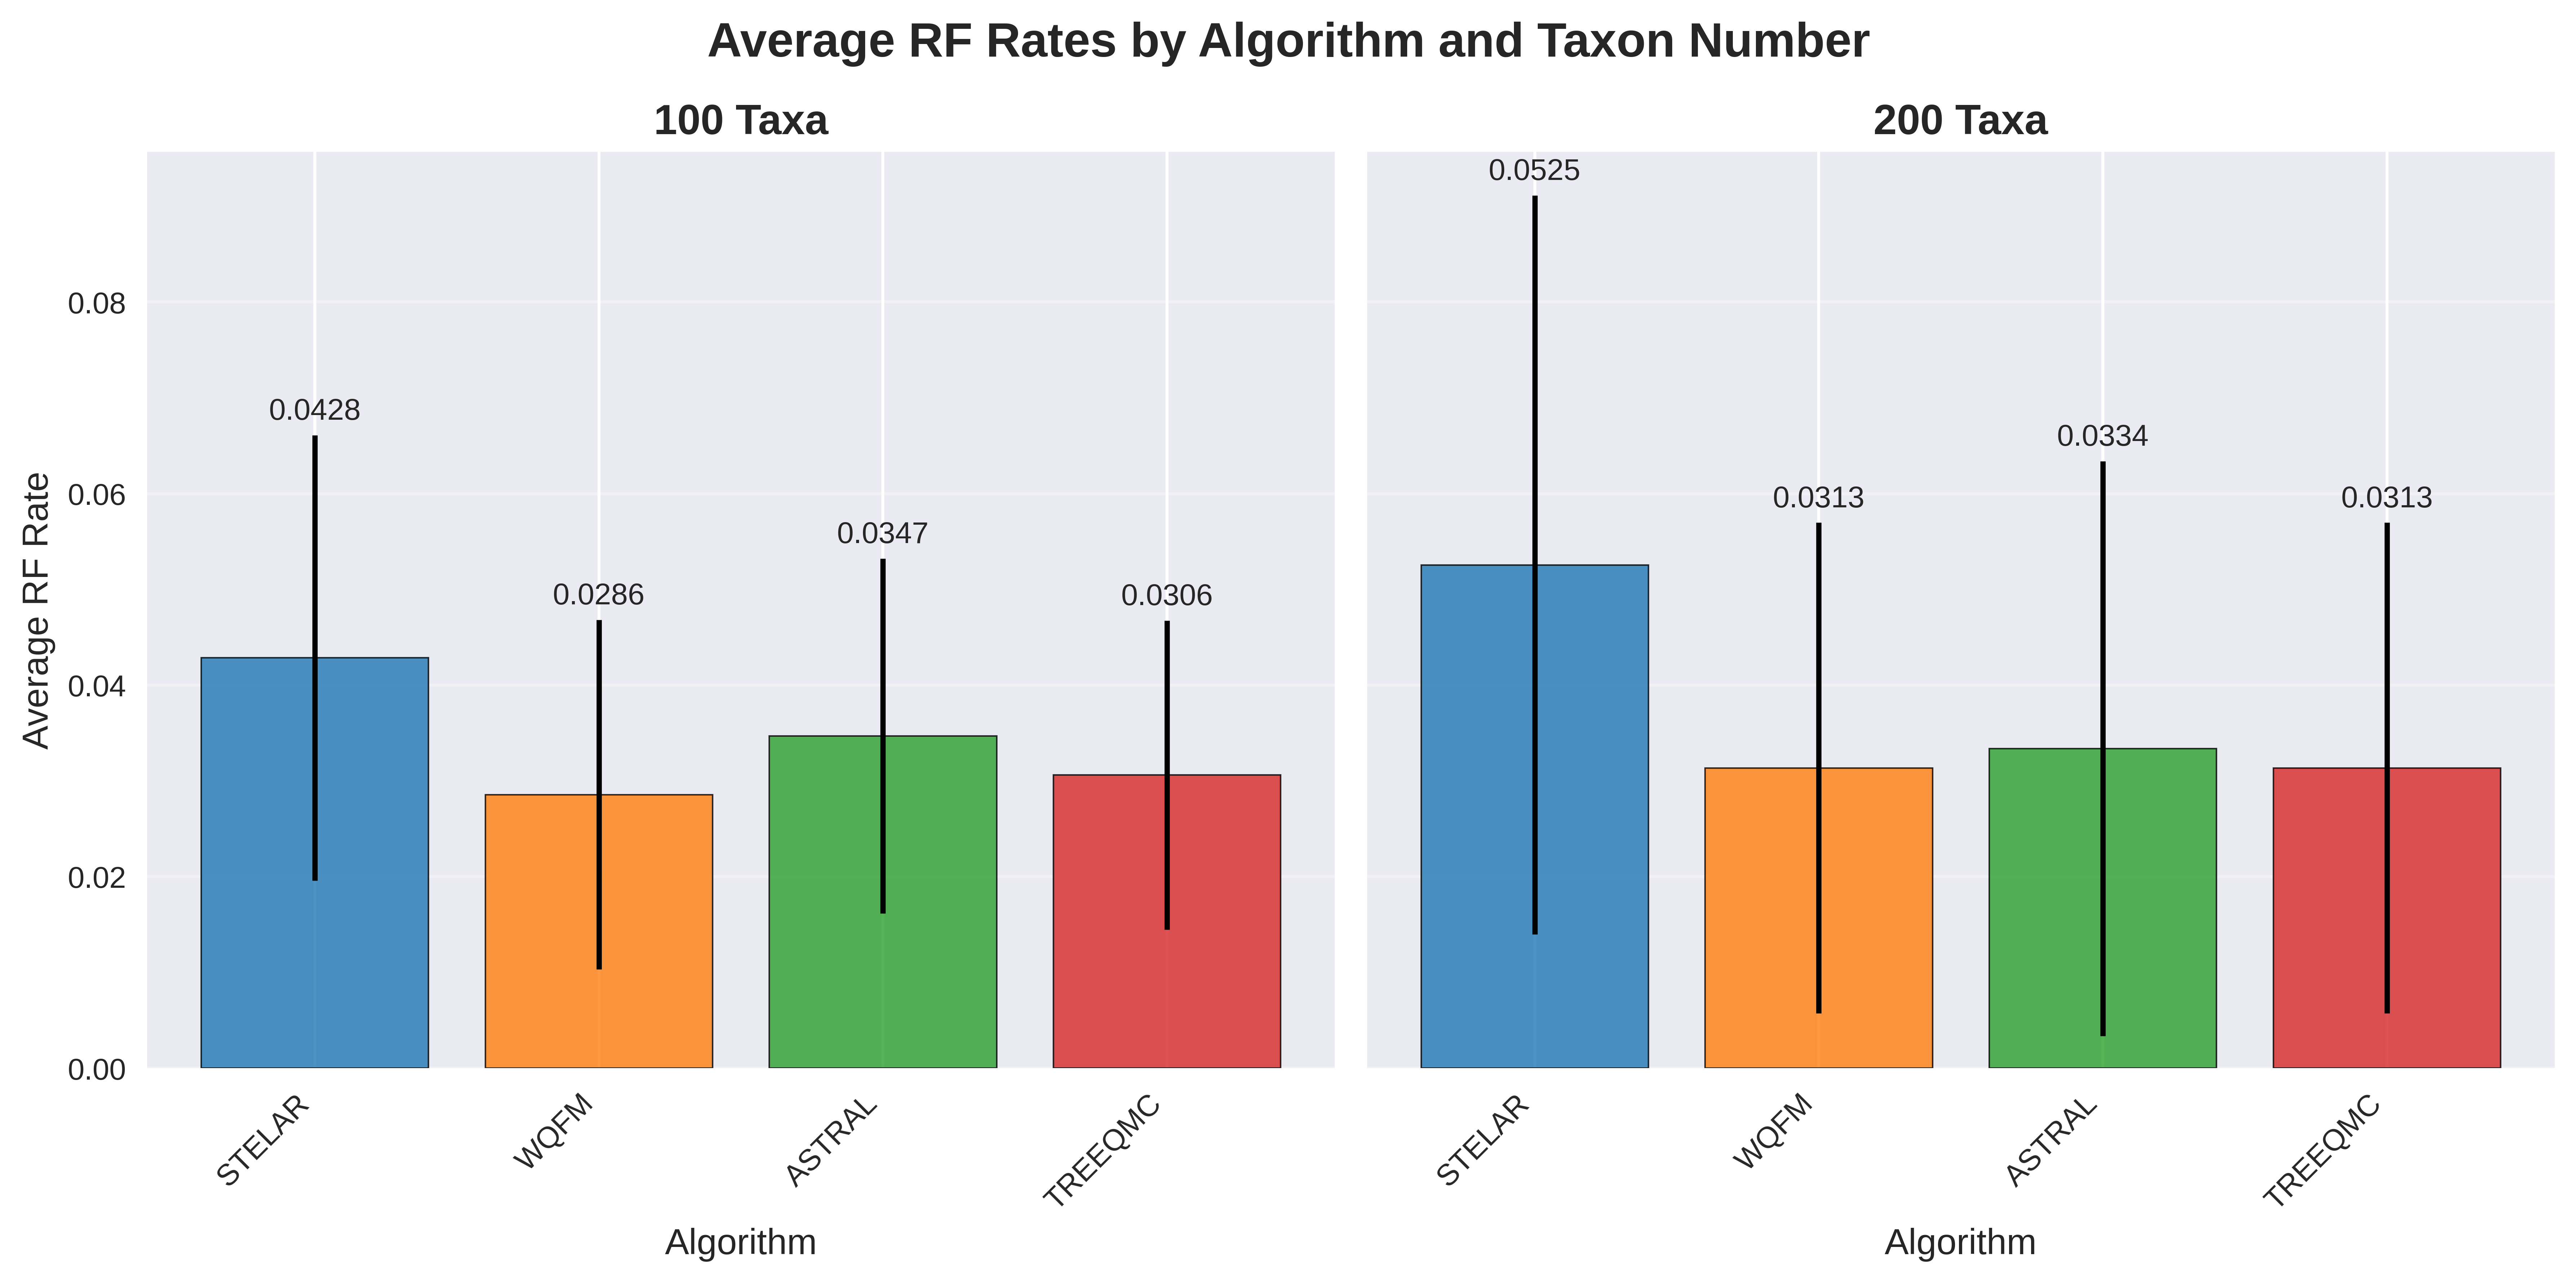
\includegraphics[width=0.8\linewidth]{fig-stx/results/rf_rates_comparison.png}
    \caption{Caption}
    \label{fig:placeholder}
\end{figure}

\subsection{Speedups in Running Time}

\begin{figure}
    \centering
    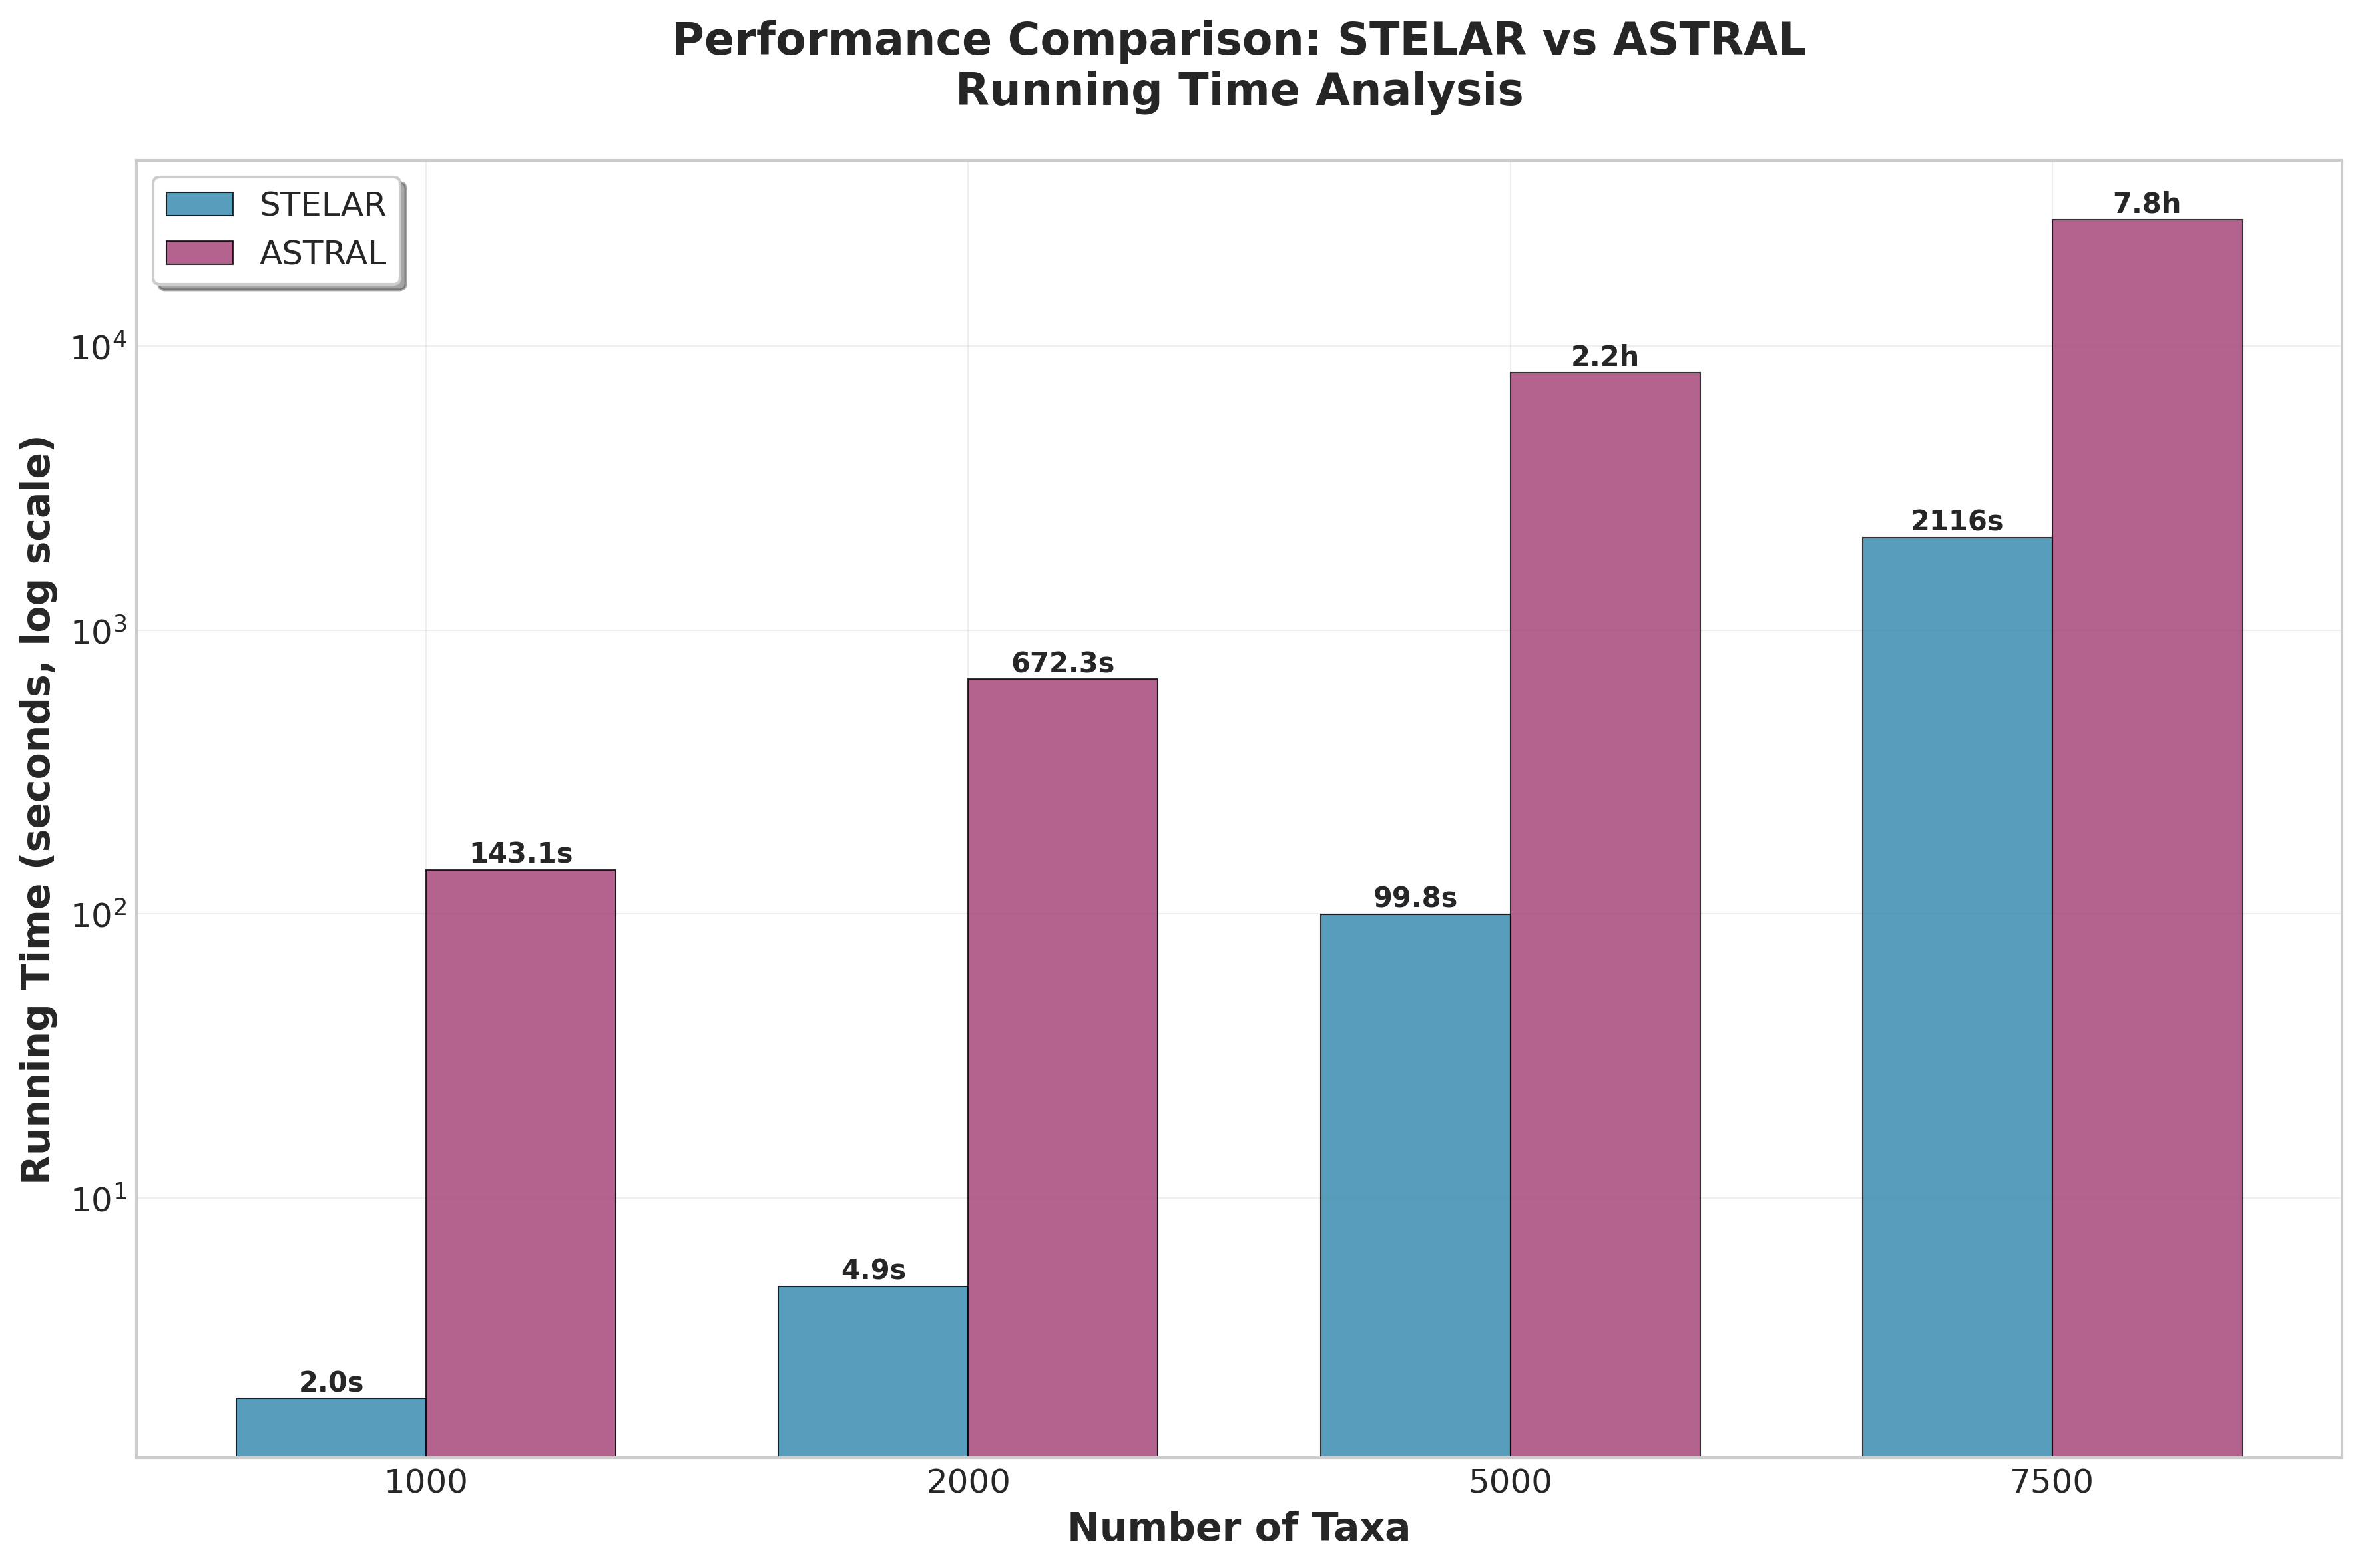
\includegraphics[width=0.75\linewidth]{fig-stx/results/time_comparison.png}
    \caption{Caption}
    \label{fig:placeholder}
\end{figure}

\subsection{Reduction in Memory Usage}

\begin{figure}
    \centering
    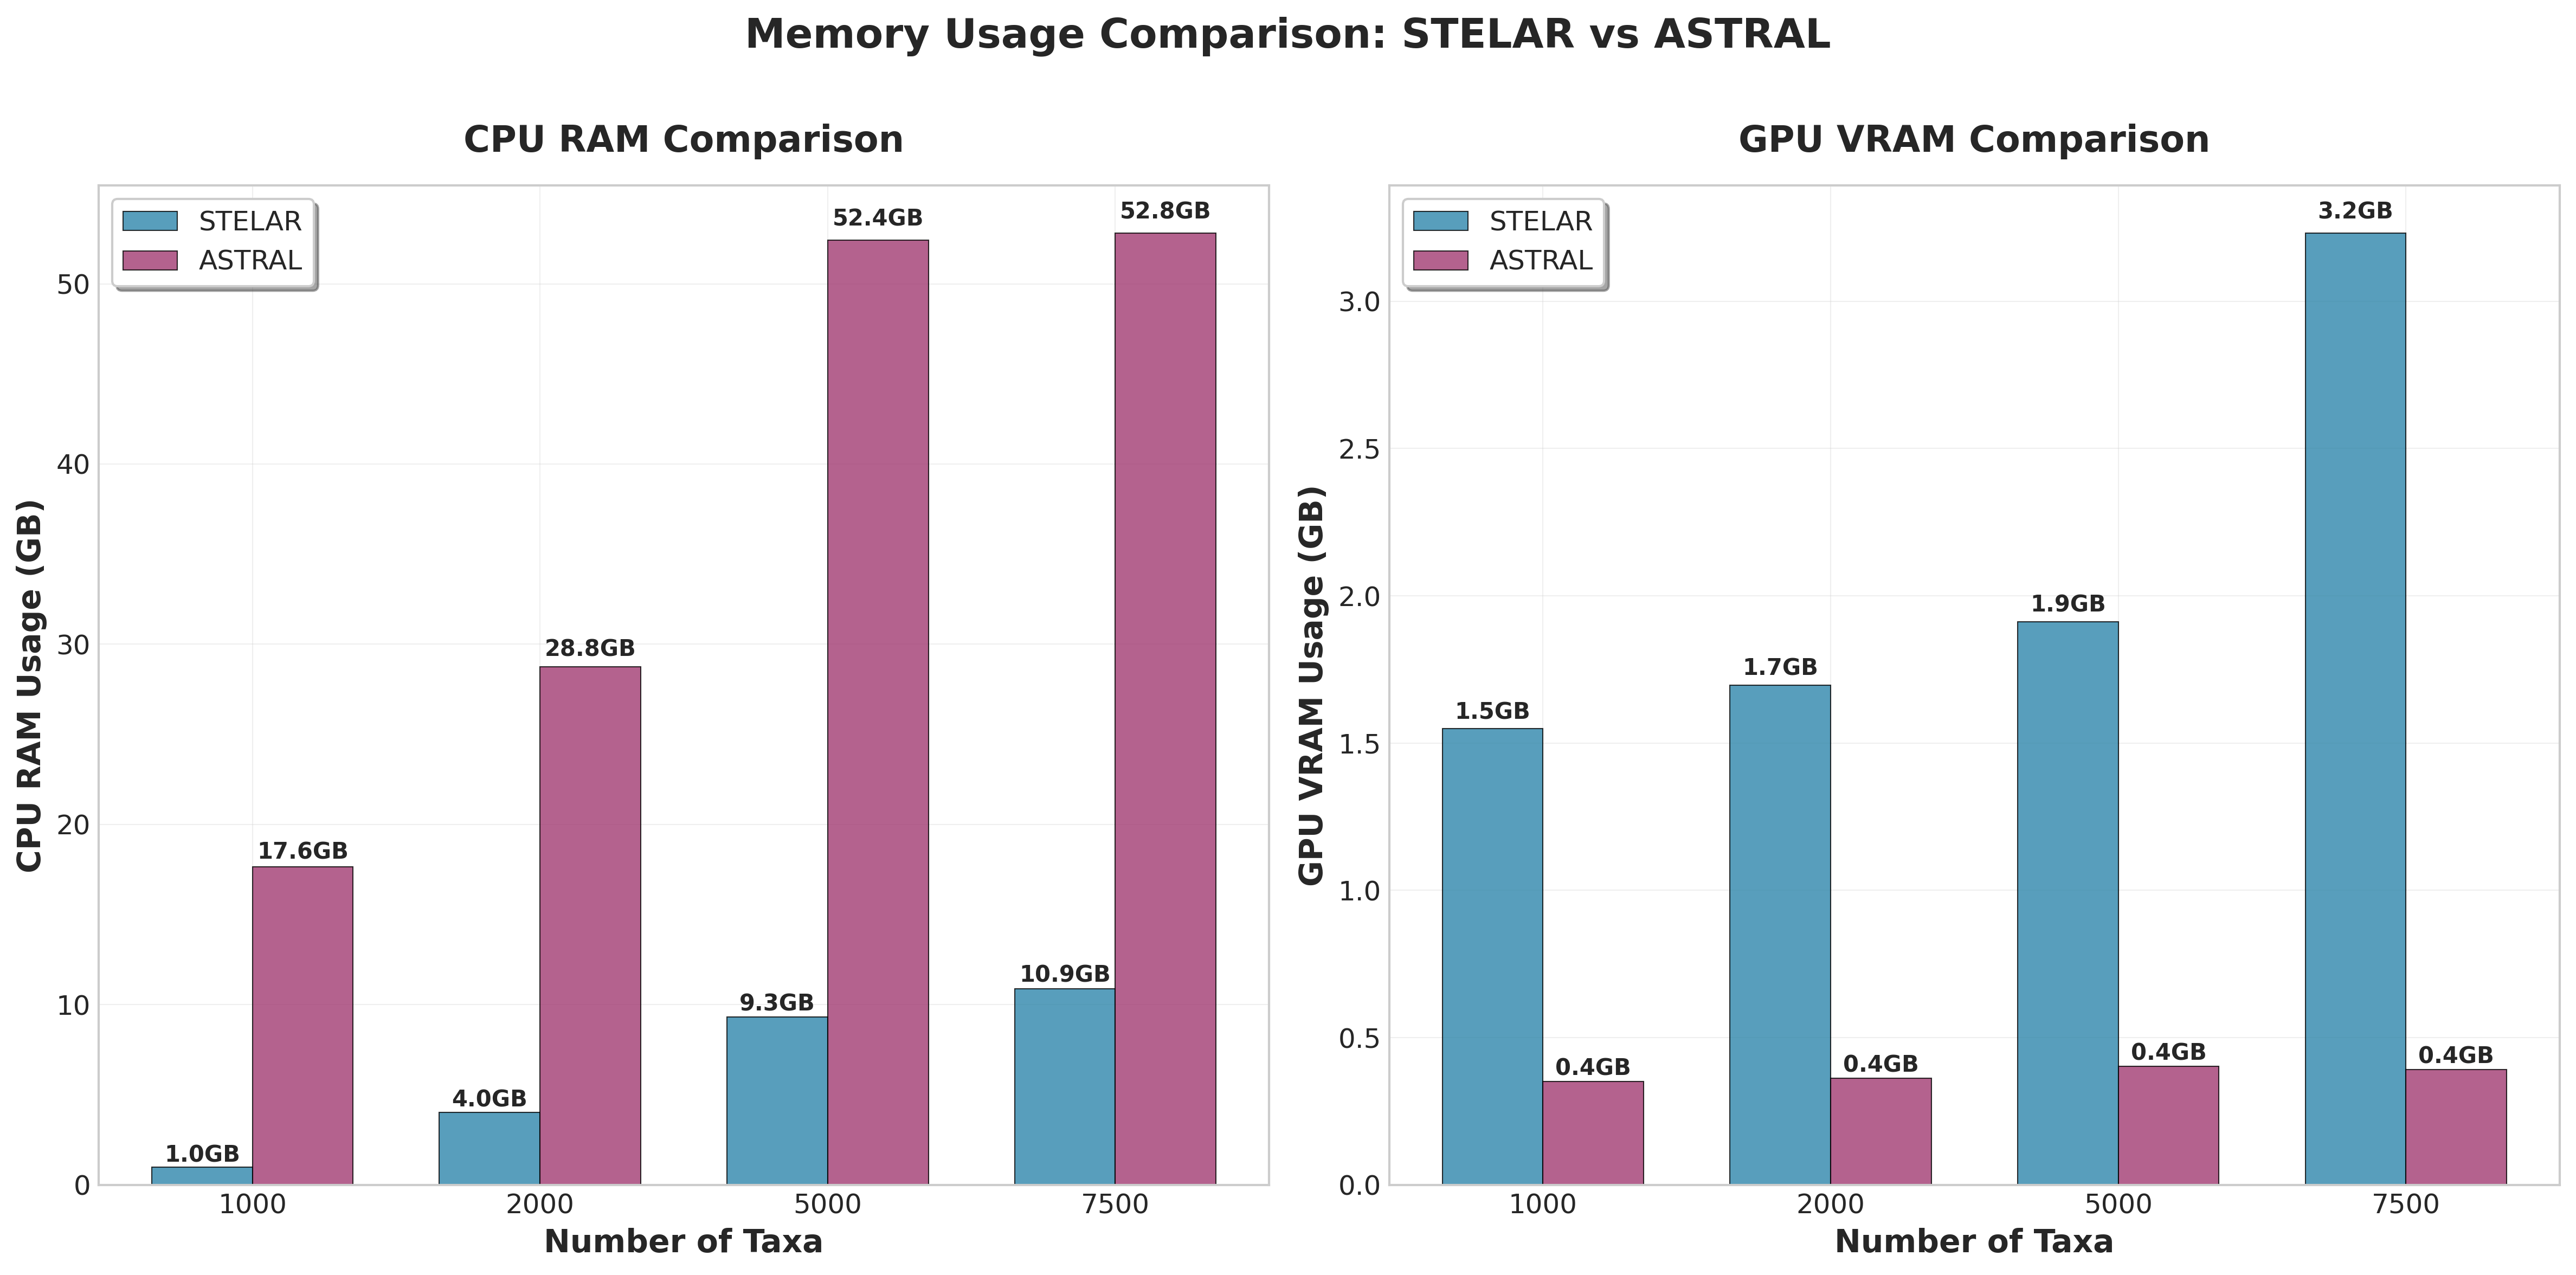
\includegraphics[width=0.9\linewidth]{fig-stx/results/memory_comparison.png}
    \caption{Caption}
    \label{fig:placeholder}
\end{figure}

\subsection{Scaling up the Number of Taxa}

\begin{figure}
    \centering
    
\includegraphics[width=\linewidth]{fig-stx/results/stelar-scale-taxa.png}
    \caption{Caption}
    \label{fig:placeholder}
\end{figure}

% \begin{table}[h]
% \caption{Running time and memory usage of STELAR with varying number of taxa}
% \centering
% \begin{tabular}{l l l l l}
% \toprule
% No. of Taxa & No. of Gene Trees & Running Time (s) & CPU RAM (MB) & GPU VRAM (MB) \\
% \midrule
% 10000  & 1000 & 87.321   & 11047.477 & 497.664 \\
% 25000  & 1000 & 1176.499   & 18659.977 & 638.976 \\
% 50000  & 1000 & 6660.976   & 54229.543 & 858.544 \\
% 75000  & 1000 & 16901.294   & 77415.117 & 1098.364 \\
% 100000  & 1000 & 30776.740   & 86336.082 & 1330.442 \\
% \bottomrule
% \end{tabular}
% \end{table}



\subsection{Scaling up the Number of Gene Trees}

\begin{figure}
    \centering
    
\includegraphics[width=\linewidth]{fig-stx/results/stelar-scale-gt-1k.png}
    \caption{Caption}
    \label{fig:placeholder}
\end{figure}

% \begin{table}[h]
% \caption{Running time and memory usage of STELAR with varying number of gene trees}
% \centering
% \begin{tabular}{l l l l l}
% \toprule
% No. of Taxa & No. of Gene Trees & Running Time (s) & CPU RAM (MB) & GPU VRAM (MB) \\
% \midrule
% 10000  & 1000 & 87.321   & 11047.477 & 497.664 \\
% 10000  & 2500 & 419.918   & 19518.605 & 624.640 \\
% 10000  & 5000 & 1291.352   & 24002.172 & 829.440 \\
% 10000  & 7500 & 2211.381   & 53890.949 & 1008.446 \\
% 10000  & 10000 & 3111.629   & 75593.758 & 1208.248 \\
% \bottomrule
% \end{tabular}
% \end{table}


\subsection{Effect of ILS on Performance}


\begin{table}[h]
\caption{Discordance levels under different ILS conditions}
\centering
\setlength{\tabcolsep}{8pt}
\begin{tabular}{l c c}
\toprule
\textbf{ILS Level} & \textbf{GT--GT Discordance (\%)} & \textbf{GT--ST Discordance (\%)} \\
\midrule
ILS-L1 & 25.4 & 17.5 \\
ILS-L2 & 31.7 & 22.1 \\
ILS-L3 & 37.5 & 26.4 \\
ILS-L4 & 42.8 & 30.7 \\
\bottomrule
\end{tabular}
\end{table}


\begin{figure}
    \centering
    
\includegraphics[width=\linewidth]{fig-stx/results/vary-ils-performance.png}
    \caption{Caption}
    \label{fig:placeholder}
\end{figure}


% \begin{table}[h]
% \caption{Running time of STELAR-X under different ILS conditions}
% \centering
% \setlength{\tabcolsep}{8pt}
% \begin{tabular}{l l c c c c}
% \toprule
% \multicolumn{2}{c}{} & \multicolumn{4}{c}{\textbf{Running Time (s)}} \\
% \cmidrule(lr){3-6}
% No. of Taxa & No. of Gene Trees & ILS-L1 & ILS-L2 & ILS-L3 & ILS-L4 \\
% \midrule
% 10000 & 1000 & 68.12 & 87.32 & 121.61 & 182.68 \\
% 15000 & 1000 & 147.25 & 200.62 & 294.76 & 443.33 \\
% 20000 & 1000 & 339.71 & 563.79 & 999.84 & 1715.54 \\
% 25000 & 1000 & 647.36 & 1176.50 & 2142.89 & 3733.87 \\
% \bottomrule
% \end{tabular}
% \end{table}

% \begin{table}[h]
% \caption{CPU RAM usage of STELAR-X under different ILS conditions}
% \centering
% \setlength{\tabcolsep}{8pt}
% \begin{tabular}{l l c c c c}
% \toprule
% \multicolumn{2}{c}{} & \multicolumn{4}{c}{\textbf{CPU RAM (MB)}} \\
% \cmidrule(lr){3-6}
% No. of Taxa & No. of Gene Trees & ILS-L1 & ILS-L2 & ILS-L3 & ILS-L4 \\
% \midrule
% 10000 & 1000 & 12123.14 & 11047.48 & 11538.92 & 12451.77 \\
% 15000 & 1000 & 16030.71 & 16413.78 & 16454.35 & 16542.80 \\
% 20000 & 1000 & 17530.17 & 18945.68 & 19319.74 & 18463.49 \\
% 25000 & 1000 & 17452.03 & 18659.98 & 19913.23 & 20318.38 \\
% \bottomrule
% \end{tabular}
% \end{table}

% \begin{table}[h]
% \caption{GPU VRAM usage of STELAR-X under different ILS conditions}
% \centering
% \setlength{\tabcolsep}{8pt}
% \begin{tabular}{l l c c c c}
% \toprule
% \multicolumn{2}{c}{} & \multicolumn{4}{c}{\textbf{GPU VRAM (MB)}} \\
% \cmidrule(lr){3-6}
% No. of Taxa & No. of Gene Trees & ILS-L1 & ILS-L2 & ILS-L3 & ILS-L4 \\
% \midrule
% 10000 & 1000 & 491.52 & 497.66 & 501.76 & 514.05 \\
% 15000 & 1000 & 534.53 & 538.62 & 550.91 & 565.25 \\
% 20000 & 1000 & 579.58 & 591.87 & 606.21 & 628.74 \\
% 25000 & 1000 & 624.64 & 638.98 & 659.46 & 681.98 \\
% \bottomrule
% \end{tabular}
% \end{table}



\begin{figure}
    \centering
    
\includegraphics[width=0.9\linewidth]{fig-stx/trees/avian-stelar-circ-normal.png}
    \caption{Caption}
    \label{fig:placeholder}
\end{figure}



\section{Discussion}

\textcolor{blue}{TODO}


\section{Conclusion}

\textcolor{blue}{TODO}


\subsection{Datasets}

\subsubsection{Simulated Datasets}

\begin{enumerate}
    \item 100-taxon, 200-taxon -> accuracy comparison among STELAR , ASTRAL, WQFM-TREE, TREE-QMC

    \item Large Simulated Datasets -> accuracy, runtime, CPU RAM, GPU VRAM

    

    
\end{enumerate}

\subsubsection{Empirical Datasets}

\begin{enumerate}
    \item 1kp plant Dataset - accuracy and runtime
\end{enumerate}

\subsection{Simulation Parameters}

\begin{table}[h!]
\centering

\begin{tabular}{|l|l|}
\hline
\textbf{Parameter Name} & \textbf{parameter Value} \\ \hline
\textbf{Speciation rate} & 0.0000001 \\ \hline
Extinsion rate & 0 \\ \hline
Number of Taxa & 100 \\ \hline
Ingroup divergence to the ingroup ratio & 1.0 \\ \hline
Generations & LogN(1.470055e+01,2.500000e-01) \\ \hline
\textbf{Haploid effective population size} & 400000 \\ \hline
Global substitution rate & LogN(-1.727461e+01,6.931472e-01) \\ \hline
Lineage specific rate gamma shape & LogN(1.500000e+00,1) \\ \hline
Gene family specific rate gamma shape & LogN(1.551533e+00,6.931472e-01) \\ \hline
Gene tree branch specific rate gamma shape & LogN(1.500000e+00,1) \\ \hline
Seed & 22 \\ \hline
% Sequence Length & 1600 \\ \hline
% Sequence base frequencies & Dirichlet(A=36,C=26,G=28,T=32) \\ \hline
% Sequence transition rates & Dirichlet(TC=16,TA=3,TG=5,CA=5,CG=6,AG=15) \\ \hline
\end{tabular}
\vspace{6pt}
\caption{Simulation parameters used for the generation of gene trees and species trees in Simphy}
\label{tab:simphy-params}

\end{table}


\bibliographystyle{unsrt}
% \bibliography{References}
\bibliographystyle{IEEEtran}
\bibliography{references.bib} % NEED TO CHANGE to references.bib

\end{document}
